% ============================================================
%  UIU CampusConnect - Project Management Report
%  Preamble
% ============================================================
\documentclass[11pt,a4paper]{report}

\usepackage[T1]{fontenc}
\usepackage[utf8]{inputenc}
\usepackage{mathptmx}
\usepackage[scaled=0.92]{helvet}
\usepackage{microtype}
\usepackage[english]{babel}

\usepackage[a4paper,top=2.5cm,bottom=2.5cm,left=2.4cm,right=2.4cm,headheight=15pt]{geometry}
\usepackage{graphicx}
\usepackage{amssymb}
\usepackage{xcolor}
\usepackage{array}
\usepackage{booktabs}
\usepackage{longtable}
\usepackage{tabularx}
\usepackage{ragged2e}
\usepackage{colortbl}
\usepackage{multirow}
\usepackage{enumitem}
\usepackage{titlesec}
\usepackage{fancyhdr}
\usepackage{caption}
\usepackage{pdflscape}
\usepackage[most]{tcolorbox}
\usepackage{forest}
\useforestlibrary{edges}
\usetikzlibrary{positioning,arrows.meta,shapes.geometric,calc}
\usepackage[hidelinks]{hyperref}

% ----------------------- Colours ---------------------------
\definecolor{uiuNavy}{HTML}{123A5F}
\definecolor{uiuBlue}{HTML}{1F5F8B}
\definecolor{uiuTeal}{HTML}{2E7D8F}
\definecolor{uiuGold}{HTML}{B8860B}
\definecolor{headRow}{HTML}{123A5F}
\definecolor{lvl1Row}{HTML}{C9D9E6}
\definecolor{lvl2Row}{HTML}{E2EBF2}
\definecolor{lvl3Row}{HTML}{F2F6F9}
\definecolor{lineGrey}{HTML}{9AA7B1}
\definecolor{softGrey}{HTML}{F4F5F7}
\definecolor{riskHigh}{HTML}{B03A2E}
\definecolor{riskMed}{HTML}{B9770E}
\definecolor{riskLow}{HTML}{1E7A46}

% ----------------------- Headings --------------------------
\titleformat{\chapter}[display]
  {\normalfont\Large\bfseries\color{uiuNavy}}
  {\filright\normalsize\sffamily\textcolor{uiuBlue}{\MakeUppercase{\chaptertitlename\ \thechapter}}}
  {6pt}
  {\huge\sffamily}
  [\vspace{2pt}{\color{uiuGold}\titlerule[1.2pt]}]
\titlespacing*{\chapter}{0pt}{-16pt}{22pt}

\titleformat{\section}
  {\normalfont\large\sffamily\bfseries\color{uiuNavy}}{\thesection}{0.7em}{}
\titleformat{\subsection}
  {\normalfont\normalsize\sffamily\bfseries\color{uiuBlue}}{\thesubsection}{0.6em}{}
\titleformat{\subsubsection}
  {\normalfont\normalsize\sffamily\bfseries\color{uiuTeal}}{\thesubsubsection}{0.6em}{}
\titlespacing*{\section}{0pt}{14pt}{6pt}
\titlespacing*{\subsection}{0pt}{11pt}{4pt}
\titlespacing*{\subsubsection}{0pt}{9pt}{3pt}

% ----------------------- Header / Footer -------------------
\pagestyle{fancy}
\fancyhf{}
\renewcommand{\headrulewidth}{0.4pt}
\renewcommand{\footrulewidth}{0pt}
\fancyhead[L]{\footnotesize\sffamily\textcolor{uiuNavy}{UIU CampusConnect}}
\fancyhead[R]{\footnotesize\sffamily\textcolor{uiuNavy}{Project Management Report}}
\fancyfoot[C]{\footnotesize\sffamily\thepage}
\fancypagestyle{plain}{%
  \fancyhf{}%
  \renewcommand{\headrulewidth}{0pt}%
  \fancyfoot[C]{\footnotesize\sffamily\thepage}%
}

% ----------------------- Float placement -------------------
\renewcommand{\topfraction}{0.92}
\renewcommand{\bottomfraction}{0.85}
\renewcommand{\textfraction}{0.08}
\renewcommand{\floatpagefraction}{0.7}
\setcounter{topnumber}{3}
\setcounter{bottomnumber}{2}
\setcounter{totalnumber}{5}

% ----------------------- Captions --------------------------
\captionsetup{font=small,labelfont={bf,sf,color=uiuNavy},textfont=sf,skip=6pt}

% ----------------------- Lists -----------------------------
\setlist[itemize]{leftmargin=1.4em,itemsep=4pt,topsep=4pt}
\setlist[enumerate]{leftmargin=1.6em,itemsep=4pt,topsep=4pt}

% ----------------------- Table helpers ---------------------
\newcolumntype{L}[1]{>{\RaggedRight\arraybackslash}p{#1}}
\newcolumntype{C}[1]{>{\Centering\arraybackslash}p{#1}}
\newcommand{\thead}[1]{\textcolor{white}{\sffamily\bfseries #1}}
\renewcommand{\arraystretch}{1.28}
\setlength{\tabcolsep}{5pt}
\arrayrulecolor{lineGrey}

% Coloured header row for tables
\newcommand{\rowhead}{\rowcolor{headRow}}

% ----------------------- Callout box -----------------------
\newtcolorbox{keybox}[1][]{%
  enhanced, breakable,
  colback=softGrey, colframe=uiuBlue,
  boxrule=0pt, leftrule=3pt,
  arc=1pt, left=8pt, right=8pt, top=6pt, bottom=6pt,
  fonttitle=\sffamily\bfseries, #1}

\newtcolorbox{riskcard}[1]{%
  enhanced, breakable,
  colback=white, colframe=uiuNavy,
  boxrule=0.7pt, arc=2pt,
  title={\sffamily\bfseries #1},
  colbacktitle=uiuNavy,
  left=8pt, right=8pt, top=6pt, bottom=6pt}

% ----------------------- WBS tree style --------------------
\forestset{
  wbstree/.style={
    for tree={
      font=\sffamily\scriptsize,
      grow'=0,
      folder,
      folder indent=1.1em,
      draw=uiuBlue,
      line width=0.4pt,
      rounded corners=1.5pt,
      inner xsep=4pt,
      inner ysep=2.2pt,
      edge={draw=lineGrey, line width=0.5pt},
      align=left,
      l sep=0.9em,
      s sep=1.6pt,
    }
  },
  lvlA/.style={fill=lvl1Row, font=\sffamily\scriptsize\bfseries},
  lvlB/.style={fill=lvl2Row, font=\sffamily\scriptsize\bfseries},
  lvlC/.style={fill=lvl3Row, font=\sffamily\scriptsize},
  lvlD/.style={fill=white, font=\sffamily\scriptsize},
}

\newcommand{\wbsfignote}[1]{\par\vspace{2pt}{\footnotesize\itshape #1\par}}

\hypersetup{
  pdftitle={UIU CampusConnect - Project Management Report},
  pdfauthor={Group 09, Section B, Department of CSE, United International University},
  pdfsubject={Vision and Scope, Methodology, Risk Management and Work Breakdown Structure}
}
\begin{document}

% ============================================================
%  COVER PAGE
% ============================================================
\begin{titlepage}
\thispagestyle{empty}
\centering
\vspace*{0.6cm}

{\color{uiuGold}\rule{\textwidth}{2.5pt}}\\[2pt]
{\color{uiuNavy}\rule{\textwidth}{0.8pt}}

\vspace{1.0cm}

{\sffamily\bfseries\Large\color{uiuNavy} UNITED INTERNATIONAL UNIVERSITY}\\[6pt]
{\sffamily\large\color{uiuBlue} Department of Computer Science \& Engineering}\\[4pt]
{\sffamily\normalsize\color{uiuTeal} School of Science \& Engineering}

\vspace{1.6cm}

{\sffamily\normalsize\color{uiuBlue}\MakeUppercase{Project Management Report}}

\vspace{0.7cm}

{\color{uiuGold}\rule{0.35\textwidth}{1.2pt}}

\vspace{0.9cm}

{\sffamily\bfseries\fontsize{34}{40}\selectfont\color{uiuNavy} UIU CampusConnect}

\vspace{0.5cm}

{\sffamily\Large\color{uiuBlue} Campus Social \& Academic Networking Platform}

\vspace{0.45cm}

{\itshape\normalsize\color{black!70} Vision \& Scope \quad\textbullet\quad Development Methodology \\[2pt]
Risk Management \& RMMM \quad\textbullet\quad Work Breakdown Structure}

\vspace{0.9cm}

{\color{uiuGold}\rule{0.35\textwidth}{1.2pt}}

\vspace{1.1cm}

{\sffamily\large\bfseries\color{uiuNavy} Team No. 09 \quad\textbar\quad Section: B}

\vspace{0.5cm}

\begin{tabular}{|>{\Centering\arraybackslash}p{1.6cm}|>{\RaggedRight\arraybackslash}p{7.2cm}|>{\Centering\arraybackslash}p{3.4cm}|}
\hline
\rowcolor{headRow}
\thead{S/N} & \thead{Name of Team Member} & \thead{Student ID} \\ \hline
1 & Sindeed Shuaib Arpon & 0112330261 \\ \hline
\rowcolor{lvl3Row}
2 & Nafiz Iqbal Razin & 0112330204 \\ \hline
3 & Afnan Zaman Mohammad Sajid & 0112330036 \\ \hline
\rowcolor{lvl3Row}
4 & Farzana Akter & 0112320101 \\ \hline
\end{tabular}

\vfill

{\sffamily\normalsize\color{uiuNavy} Date of Submission: \today}

\vspace{0.5cm}
{\color{uiuNavy}\rule{\textwidth}{0.8pt}}\\[2pt]
{\color{uiuGold}\rule{\textwidth}{2.5pt}}

\end{titlepage}

% ============================================================
%  TABLE OF CONTENTS
% ============================================================
\pagenumbering{roman}
\setcounter{page}{1}
{\hypersetup{linkcolor=black}
\tableofcontents}
\clearpage
\pagenumbering{arabic}
\setcounter{page}{1}

% ============================================================
\chapter{Introduction}
% ============================================================

\section{Project Overview}

UIU CampusConnect is a university-focused digital platform that brings social
networking, academic communication, campus notices, events, clubs, peer-to-peer
services and administrative functions into a single shared environment. At
present a student at United International University has to move between a
notice board, a departmental portal, several unofficial Facebook groups, a
handful of WhatsApp or Messenger threads and word-of-mouth in order to keep
track of what is happening on campus. Information is duplicated, arrives late,
and is frequently impossible to verify. CampusConnect exists to remove that
fragmentation.

The platform is built around role-based authentication, personalised feeds,
profiles, private messaging, notifications, official notices, academic section
announcements, events with registration and QR check-in, club management, course
and project groups, a campus marketplace, lost-and-found, global search,
moderation and system administration. Every one of these modules is treated as a
managed deliverable in this report: it is scoped in Chapter~\ref{ch:vision},
scheduled through the methodology described in Chapter~\ref{ch:method}, protected
by the risk plan in Chapter~\ref{ch:risk}, and decomposed into work packages in
Chapter~\ref{ch:wbs}.

\section{Purpose and Structure of this Report}

This document is the consolidated project management report for UIU
CampusConnect. It is not a design specification and it is not a user manual; it
records the management decisions that govern how the system will be built, by
whom, in what order, at what cost, and with what protection against failure. The
report is organised as follows.

\begin{itemize}
  \item \textbf{Chapter~\ref{ch:vision} -- Vision and Scope} fixes the boundary
  of the product. It states what CampusConnect is for, lists the objectives it
  must achieve, defines the functional areas that are inside the delivery
  boundary, and explicitly records what the team will \emph{not} build.
  \item \textbf{Chapter~\ref{ch:method} -- Development Methodology} compares the
  candidate process models against the actual characteristics of this project,
  justifies the selection of Agile Scrum, gives a reasoned explanation of why
  each alternative was set aside, and shows how Scrum ceremonies map onto the
  CampusConnect modules.
  \item \textbf{Chapter~\ref{ch:wbs} -- Work Breakdown Structure} decomposes the
  entire scope into four hierarchical levels, from the platform itself down to
  individually assignable work packages, with effort allocations that roll up to
  100\% of the project.
  \item \textbf{Chapter~\ref{ch:delphi} -- Wideband Delphi Estimation} converts
  that structure into absolute effort. Five estimators worked through three
  rounds of consensus estimation; the chapter records every round, analyses how
  the estimates converged, and works one feature's estimation session through in
  full.
  \item \textbf{Chapter~\ref{ch:risk} -- Risk Management and RMMM} identifies
  the risks that threaten the platform, defines the team's Risk Mitigation,
  Monitoring and Management procedure, works three representative risks through
  that procedure in full, and consolidates all identified risks into a risk plan
  sheet.
\end{itemize}

% ============================================================
\chapter{Vision and Scope}
\label{ch:vision}
% ============================================================

\section{Vision Statement}

\begin{keybox}
To create a unified digital campus ecosystem that connects students, faculty,
university officials and campus organisations through social interaction,
academic collaboration, communication and community services.
\end{keybox}

Each clause of this statement carries a concrete obligation for the CampusConnect
build. \emph{Unified} means that a student signs in once and reaches notices,
sections, clubs, events and peers from a single feed, rather than maintaining
accounts on several disconnected services. \emph{Digital campus ecosystem} means
the platform mirrors the real structure of the university -- departments,
sections, batches, clubs and offices are first-class entities in the data model,
not free-text labels. \emph{Connects students, faculty, university officials and
campus organisations} is the reason the system is role-based from the very first
sprint: a notice published by the Registrar's office must be visibly different
from a post written by a classmate, and the platform must be able to prove which
is which. Finally, \emph{social interaction, academic collaboration,
communication and community services} names the four pillars that later become
the top-level branches of the Work Breakdown Structure in Chapter~\ref{ch:wbs}.

\section{Project Objectives}

The vision is delivered through six measurable objectives. Each objective below
is stated first, then explained in terms of the specific CampusConnect features
that satisfy it.

\subsection*{O1. Improve the speed and reach of university communication}

Official information at UIU currently travels through physical notice boards,
email and informal re-sharing, which means a student who misses one channel
misses the announcement entirely. CampusConnect replaces that with the
\emph{Official University Notice Board}, where an authorised office publishes
once and the notice is targeted to the exact audience it concerns -- a
department, a batch, a section or the whole campus -- and is pushed instantly
through the notification centre. Because notices are stored, tagged by priority
and searchable, reach is no longer dependent on a student being online at the
moment of publication. This objective is realised by WBS elements 4.1.1 and
2.2.2.

\subsection*{O2. Provide a campus-specific social and networking environment}

General-purpose social networks mix campus life with unrelated content and admit
anyone. CampusConnect restricts registration to verified university email
addresses, so every account belongs to a real member of the UIU community. On
top of that trusted membership the platform provides the campus feed, posts with
rich media, reactions, comments, polls and saved content -- the same social
affordances students already expect, but scoped to people they actually share a
campus with. This objective is realised by WBS elements 2.1.1, 3.1 and 3.2.

\subsection*{O3. Support academic interaction between students and faculty}

Academic contact today depends on catching a teacher in the corridor or hoping a
reply arrives by email. CampusConnect gives faculty structured profiles carrying
office hours, course allocation and research interests, and gives every course
section a channel through which the assigned teacher can post announcements that
reach exactly the enrolled students. Course, batch and project groups extend the
same idea to peer learning, with a shared file area for slides, notes and
project documents. This objective is realised by WBS elements 2.1.2, 4.1.2 and
4.3.2.

\subsection*{O4. Centralise events, clubs, notices and community activities}

Club recruitment, seminars, workshops and cultural events are currently
advertised in whichever group the organiser happens to have access to, and
attendance is counted on paper. CampusConnect provides a single events module
with publishing, capacity limits, interested/going responses, registration and
QR-token check-in, together with a club directory in which every registered club
maintains its own profile, membership list, content and gallery. The result is
one authoritative campus calendar and one verifiable attendance record. This
objective is realised by WBS elements 4.2 and 4.3.1.

\subsection*{O5. Provide peer-to-peer services such as marketplace and lost-and-found}

Students routinely resell textbooks, calculators and lab equipment, and lose
belongings on campus, but have no trusted place to do either. CampusConnect adds
a campus marketplace where verified students list items with photographs,
category and price and mark them sold when the exchange is complete, and a
lost-and-found register where a finder posts an item and a claimant must supply
identifying details before the claim is released. Because both services run on
top of verified identities, the platform can attribute every listing and claim to
a real student, which is precisely what makes them safer than an anonymous
group. This objective is realised by WBS element 5.1.

\subsection*{O6. Maintain role-based security, moderation and administrative control}

A platform that carries official notices, private messages and personal profiles
cannot be governed informally. CampusConnect enforces a permission matrix in
which student, faculty, official and administrator roles each see and do only
what their role allows; provides a reporting mechanism and a moderation centre
where flagged content is reviewed and actioned; and gives administrators a
dashboard with immutable audit logs of every privileged action. This objective is
what makes the other five safe to deploy, and it is realised by WBS elements
2.1.1, 5.2 and 1.3.1.

\section{In-Scope Functional Areas}

Table~\ref{tab:inscope} defines the delivery boundary of the project. The first
two columns state the functional area and the functionality it contains; the
third column explains why that area belongs in CampusConnect, so that the scope
can be defended when new requests arrive during development.

\begin{longtable}{|L{2.6cm}|L{5.1cm}|L{6.2cm}|}
\caption{In-scope functional areas of UIU CampusConnect and their justification}
\label{tab:inscope}\\
\hline
\rowhead \thead{Area} & \thead{Included Functionality} & \thead{Role in the CampusConnect Project} \\ \hline
\endfirsthead
\hline
\rowhead \thead{Area} & \thead{Included Functionality} & \thead{Role in the CampusConnect Project} \\ \hline
\endhead
\hline
\multicolumn{3}{r}{\footnotesize\itshape continued on next page}\\
\endfoot
\hline
\endlastfoot

\textbf{User management} &
Registration, authentication, role-based permissions, profiles and privacy
controls. &
The trust anchor of the whole platform. Restricting sign-up to university email
domains is what separates CampusConnect from an open social network, and the
role assigned at registration decides whether a user may publish an official
notice, moderate content or only participate. Nothing else can be built safely
until this is in place, so it is the first module scheduled. \\ \hline

\rowcolor{lvl3Row}
\textbf{Social networking} &
Campus feed, personalised views, posts, media, reactions, comments, polls and
saved content. &
The layer that gives students a reason to open the application daily. A
personalised feed mixing department, batch and followed sources keeps the
platform relevant to each individual, while polls and saved content turn passive
reading into participation and let clubs and class representatives gather
opinion quickly. \\ \hline

\textbf{Communication} &
Connections, following, private messaging and notifications. &
Replaces the scattered Messenger and WhatsApp threads students currently use for
coursework coordination. Because messaging sits inside a verified campus
identity system, a student can be certain who they are talking to, and the
central notification service ensures that a notice, an event reminder and a
message all reach the user through one consistent channel. \\ \hline

\rowcolor{lvl3Row}
\textbf{Academic support} &
Faculty profiles, office hours, research/course information, academic resources
and section announcements. &
Turns the platform from a social product into an academic one. Section-level
announcements guarantee that a change of class time or an assignment deadline
reaches every enrolled student and no one else, and published office hours
reduce the repeated individual queries that faculty currently receive. \\ \hline

\textbf{Official communication} &
Authorised university notices with targeting, priority and filtering. &
Gives the university itself a stake in the system. Only accounts with the
official role may publish here, which makes the notice board authoritative and
prevents the rumour-driven misinformation that circulates in unofficial student
groups before examinations and registration. \\ \hline

\rowcolor{lvl3Row}
\textbf{Events} &
Event publishing, registration, interest/going actions, capacity and
QR/token-based check-in. &
Solves a real operational problem for club organisers and the Office of Student
Affairs: knowing in advance how many people will attend, enforcing venue
capacity, and recording attendance without paper sign-in sheets. QR check-in
also produces the participation data clubs need for their annual reports. \\ \hline

\textbf{Clubs} &
Club directory, membership requests, club content, events and galleries. &
UIU's clubs are a major part of campus life but have no permanent online
presence. Giving each club a managed profile with a membership workflow means
recruitment, announcements and archives survive the annual change of committee
instead of disappearing with a graduating panel. \\ \hline

\rowcolor{lvl3Row}
\textbf{Groups \& resources} &
Course, batch, project and community groups with shared files. &
Supports the collaborative work that dominates a CSE student's semester. A
project group with a shared file area and a discussion board keeps code
documents, reports and decisions in one place, which is where most team
coursework currently breaks down. \\ \hline

\textbf{Community services} &
Marketplace and lost-and-found functionality. &
The peer-to-peer services of objective O5. They are deliberately in scope
because they generate everyday, non-academic reasons to return to the platform,
which is what sustains adoption after the novelty of launch. \\ \hline

\rowcolor{lvl3Row}
\textbf{Search \& moderation} &
Global search, reporting, moderation centre and administrator controls. &
The governance layer. Global search makes the accumulated notices, events and
listings retrievable rather than merely chronological, while reporting and
moderation give the team a defined response path when a user posts abusive
content or a fraudulent marketplace listing. \\ \hline

\end{longtable}

\section{Out-of-Scope Items}

The following capabilities are explicitly excluded from this release. Recording
them here is a scope-control measure: it gives the project manager a written
basis for refusing late additions, which is the main defence against the scope
creep risk registered as R9 in Chapter~\ref{ch:risk}.

\begin{itemize}
  \item \textbf{Full Learning Management System replacement.} CampusConnect
  carries section announcements and shared group files, but it will not host
  graded assignment submission, grade books or course content delivery. UIU
  already operates an LMS for that purpose, and reproducing it would multiply
  the project's size while duplicating a system the university has no intention
  of retiring.

  \item \textbf{Online examination and proctoring system.} Examinations demand
  identity assurance, secure browser control, invigilation and legally
  defensible audit trails. These requirements are of a different order from
  social and communication features, and attempting them within a student
  project timeline would put the delivery of the entire platform at risk.

  \item \textbf{Video-conferencing platform.} Real-time audio and video demands
  media servers, bandwidth provisioning and continuous operational cost.
  CampusConnect therefore supports scheduling and announcing an online session
  and linking out to an existing conferencing tool, rather than transporting the
  media itself.

  \item \textbf{University-wide ERP or finance system replacement.} Admissions,
  payroll, accounts and academic records remain in the university's existing
  administrative systems. CampusConnect may consume identity and section data
  from them, but it does not become the system of record for institutional data.

  \item \textbf{Direct financial transaction processing and payment gateway
  services.} The marketplace connects a buyer and a seller and lets them mark an
  item sold; money changes hands offline. Handling payments would bring
  PCI-DSS-level compliance obligations, chargeback handling and custody of funds
  into a student project, which is neither necessary for the objective nor
  responsibly achievable within it.
\end{itemize}

\section{Assumptions and Constraints}

The scope above is valid only while the following assumptions hold, and it is
bounded by the constraints listed with them.

\begin{itemize}
  \item \textbf{Assumption -- institutional email verification is available.}
  Role-based access depends on being able to verify a \texttt{@uiu.ac.bd} or
  \texttt{@bscse.uiu.ac.bd} address at registration. If that check is
  unavailable, the fake-account risk (R5) rises sharply and a manual approval
  step must be added.
  \item \textbf{Assumption -- section and club data can be obtained.} Section
  announcements and club directories assume the team can import, or manually
  seed, an accurate list of sections, courses and registered clubs.
  \item \textbf{Constraint -- academic calendar.} The project is executed inside
  a single semester by a four-member team, which caps total available effort and
  is the reason the WBS enforces small, individually ownable work packages.
  \item \textbf{Constraint -- no operational budget.} Deployment targets
  free or low-cost hosting tiers, which directly shapes the horizontal-scaling
  mitigation chosen for the peak-load risk (R3).
\end{itemize}
% ============================================================
\chapter{Development Methodology}
\label{ch:method}
% ============================================================

\section{Selecting a Process Model for CampusConnect}

A software methodology is the organised way in which a team moves a product from
an idea to a working, maintained system. The choice is not academic: it fixes how
requirements are captured, how often working software appears, how change is
absorbed and how risk is discovered. For CampusConnect three project
characteristics dominate the decision.

\begin{enumerate}
  \item \textbf{The requirements will move.} The platform serves students,
  faculty, club organisers and administrative offices, and none of these groups
  can fully specify what they want before they see it. A model that freezes
  requirements before construction would guarantee that the delivered system is
  the wrong one.
  \item \textbf{The system is modular but interdependent.} Ten functional areas
  can largely be built in parallel, yet they all sit on the same identity,
  notification and moderation foundations. The process must therefore allow
  parallel work while forcing frequent integration.
  \item \textbf{Effort is fixed and small.} Four students working across one
  semester cannot absorb a heavy documentation overhead, and cannot recover from
  discovering a fundamental defect late.
\end{enumerate}

\section{Comparison of Candidate Methodologies}

Table~\ref{tab:method} evaluates the four candidate models against those three
characteristics.

\begin{longtable}{|L{2.1cm}|L{3.5cm}|L{3.3cm}|L{4.6cm}|}
\caption{Candidate process models assessed against the needs of UIU CampusConnect}
\label{tab:method}\\
\hline
\rowhead \thead{Model} & \thead{Core Idea} & \thead{Principal Limitation} & \thead{Fit for CampusConnect} \\ \hline
\endfirsthead
\hline
\rowhead \thead{Model} & \thead{Core Idea} & \thead{Principal Limitation} & \thead{Fit for CampusConnect} \\ \hline
\endhead
\hline
\multicolumn{4}{r}{\footnotesize\itshape continued on next page}\\
\endfoot
\hline
\endlastfoot

\textbf{Waterfall} &
Strictly sequential phases -- requirements, design, implementation, testing,
deployment, maintenance -- with no return to a completed phase. Produces heavy,
complete documentation. &
Rigid. Change after sign-off is expensive, and testing happens so late that
major defects surface when there is no time to absorb them. &
\textbf{Rejected.} It would require students, faculty and the administration to
agree a complete specification for ten modules before any code exists, and would
leave the first working demonstration until the end of the semester. \\ \hline

\rowcolor{lvl3Row}
\textbf{Prototype} &
Build a simplified but functional model of the system, show it to users, collect
feedback and refine until the requirements are understood. &
It is a requirements-elicitation technique, not a complete construction process;
it has no built-in answer for scheduling, integration or release. &
\textbf{Partially adopted.} Prototyping is genuinely useful for the feed and
event check-in interfaces, so it is used \emph{inside} sprints as a design
activity, not as the overall project model. \\ \hline

\textbf{Spiral} &
Repeated cycles of planning, risk analysis, engineering and evaluation, with an
explicit risk-driven decision at every turn. &
Costly and heavy to administer; the ceremony only pays for itself when the
consequences of failure are severe. &
\textbf{Rejected as the overall model.} CampusConnect is risk-aware but not
safety-critical or contractually exposed. Its risk discipline is instead
supplied by the RMMM process of Chapter~\ref{ch:risk}, executed inside sprints. \\ \hline

\rowcolor{lvl3Row}
\textbf{Agile Scrum} &
Iterative and incremental delivery in short sprints from a prioritised product
backlog, with defined roles and ceremonies and working software as the measure
of progress. &
Requires committed, reasonably skilled participation from everyone, and can
invite scope creep if the backlog is not controlled. &
\textbf{Selected.} It matches all three project characteristics: it expects
changing requirements, forces integration every sprint, and produces something
demonstrable long before the deadline. \\ \hline

\end{longtable}

\section{Selected Methodology: Agile Scrum}

Agile Scrum is adopted as the development methodology for UIU CampusConnect. The
decision rests on four properties of Scrum, each of which answers a specific
problem in this project.

\begin{description}[leftmargin=0pt,style=unboxed,itemsep=6pt]
  \item[Short, timeboxed sprints.] Work is delivered in two-week sprints. Within
  one semester this yields roughly six sprints, so the team reaches a
  demonstrable, testable increment of CampusConnect within the first month
  rather than at the end. A defect in the authentication or notification
  foundation is therefore discovered while there is still time to correct it.

  \item[A prioritised product backlog.] The ten functional areas are not equally
  urgent. The backlog lets the team build authentication, profiles and the feed
  first because everything else depends on them, and defer the marketplace and
  lost-and-found until the core is stable -- without ever pretending that the
  deferred items have been forgotten.

  \item[Frequent stakeholder feedback.] Each sprint ends with a demonstration to
  the supervising faculty member and to sample users drawn from the student body
  and club committees. Questions such as whether a notice should be filtered by
  department or by section are answered by people who will actually use the
  system, in the sprint after they are raised.

  \item[Clear ownership through defined roles.] With only four members, ambiguity
  about who owns a module is fatal. Scrum's role structure, combined with the
  single-point accountability rule applied in the WBS, ensures every work
  package has exactly one owner.
\end{description}

\subsection{Scrum Roles in Team 09}

\begin{table}[htbp]
\centering
\caption{Allocation of Scrum roles within the CampusConnect team}
\label{tab:roles}
\begin{tabular}{|L{3.4cm}|L{5.0cm}|L{6.0cm}|}
\hline
\rowhead \thead{Role} & \thead{Responsibility} & \thead{Application in CampusConnect} \\ \hline
Product Owner & Owns and orders the backlog; represents the users. &
Collects requirements from students, club representatives and the supervising
faculty member, and decides sprint-by-sprint which of the ten modules is next. \\ \hline
\rowcolor{lvl3Row}
Scrum Master & Facilitates ceremonies and removes impediments. &
Runs the daily stand-up and the retrospective, and maintains the risk register
described in Chapter~\ref{ch:risk}, escalating any risk whose exposure rises. \\ \hline
Development Team & Designs, builds, integrates and tests the increment. &
All four members; each takes ownership of specific WBS work packages and is
accountable for their integration and testing. \\ \hline
\end{tabular}
\end{table}

\subsection{Applying the Scrum Cycle to UIU CampusConnect}

\begin{table}[htbp]
\centering
\caption{Scrum activities mapped onto the CampusConnect development cycle}
\label{tab:scrumcycle}
\begin{tabular}{|L{3.4cm}|L{11.0cm}|}
\hline
\rowhead \thead{Activity} & \thead{Application to UIU CampusConnect} \\ \hline
Product Backlog &
Collect and prioritise platform requirements -- authentication, profiles, feed,
messaging, notifications, notices, events, clubs, groups, marketplace,
lost-and-found, search and moderation -- expressed as user stories with
acceptance criteria and traced to WBS codes. \\ \hline
\rowcolor{lvl3Row}
Sprint Planning &
Select a realistic group of high-priority backlog items for the next two-week
sprint, sized against the 8--40 hour work packages defined in the WBS, and agree
the sprint goal. \\ \hline
Development Sprint &
Design, code, integrate and test the selected features. Every merge runs the
automated test suite from WBS 1.2.2 so that integration defects surface within
the sprint rather than at the end of the project. \\ \hline
\rowcolor{lvl3Row}
Daily Scrum &
A fifteen-minute stand-up covering progress, plan and impediments. New risks
raised here are added to the risk register the same day. \\ \hline
Sprint Review &
Demonstrate completed functionality to the supervising faculty member and a
sample of student users, and record their feedback as new or re-prioritised
backlog items. \\ \hline
\rowcolor{lvl3Row}
Sprint Retrospective &
Identify what worked, what did not, and one concrete process improvement for the
next sprint. Realised risks are reviewed here and their mitigation strategies
updated. \\ \hline
Release / Increment &
Deploy the stable, tested increment to the staging environment, update the
backlog with new learning, and re-baseline the remaining effort against the WBS. \\ \hline
\end{tabular}
\end{table}

\subsection{Indicative Sprint Roadmap}
\label{sec:roadmap}

Table~\ref{tab:roadmap} shows how the WBS modules of Chapter~\ref{ch:wbs} are
distributed across the semester. The ordering is driven by dependency:
foundations first, then the modules that consume them.

\begin{table}[htbp]
\centering
\caption{Indicative sprint roadmap for UIU CampusConnect}
\label{tab:roadmap}
\begin{tabular}{|C{1.5cm}|L{5.6cm}|L{7.3cm}|}
\hline
\rowhead \thead{Sprint} & \thead{Primary WBS Coverage} & \thead{Sprint Goal} \\ \hline
1 & 1.1, 1.2.1 & Architecture, data model, UI design system and a working build
pipeline. \\ \hline
\rowcolor{lvl3Row}
2 & 2.1 & Verified registration, login, role permissions and student/faculty
profiles. \\ \hline
3 & 3.1, 3.2.1 & Campus feed with post creation, media and visibility scoping. \\ \hline
\rowcolor{lvl3Row}
4 & 2.2, 3.2.2, 3.2.3 & Messaging, notification centre, reactions, polls and
threaded comments. \\ \hline
5 & 4.1, 4.2 & Official notice board, section announcements, events and QR
check-in. \\ \hline
\rowcolor{lvl3Row}
6 & 4.3, 5.1 & Clubs, academic groups, marketplace and lost-and-found. \\ \hline
7 & 5.2, 1.2.2, 1.3 & Moderation, admin dashboard, load testing, security audit
and deployment. \\ \hline
\end{tabular}
\end{table}


\section{Why the Other Methodologies Were Not Chosen}

Selecting Agile Scrum is only half of the decision; the other half is being able
to state why each alternative was set aside. The four subsections below give that
reasoning in terms of UIU CampusConnect rather than in the abstract.

\subsection{Why not Waterfall}

Waterfall would require the team to freeze a complete requirements specification
for all ten functional areas before writing any code, and to accept that no phase
could be revisited once signed off. Three properties of this project make that
untenable.

First, the requirements genuinely are not knowable in advance. Whether a section
announcement should reach the whole department or only the enrolled students,
whether marketplace listings should expire automatically, and how aggressively the
feed should rank departmental content are all questions that our sprint reviewers
answered only after using a working screen. Under Waterfall those answers would
arrive after the design phase had closed, and changing them would mean formal
rework of documents that were already approved.

Second, Waterfall places testing at the end. For a platform whose highest-exposure
risks are a privacy breach, a peak-load failure and silent module integration
defects (risks R1, R3 and R8 in Chapter~\ref{ch:risk}), discovering any of them in
a final test phase would leave no time in a single semester to correct them.

Third, Waterfall's strength -- heavy, complete documentation and a fixed
contractual baseline -- buys us nothing here. There is no external client, no
fixed-price contract and no regulatory approval gate that would justify the
documentation overhead for a four-member student team.

Waterfall would be the correct choice for a project whose requirements are
genuinely stable and externally fixed. CampusConnect is the opposite of that.

\subsection{Why not the Prototype model}

The Prototype model is attractive at first glance because CampusConnect is a
heavily user-facing product and we do intend to put screens in front of students
early. The problem is that prototyping is a \emph{requirements elicitation
technique}, not a complete development process. It tells the team how to discover
what users want; it says nothing about how to schedule twelve components across a
semester, how to integrate the work of four people, when to test, or when to
release.

Used as the overall model it also carries two specific dangers for this project.
Because a prototype is deliberately built to be thrown away or reworked, teams
under deadline pressure frequently promote a prototype into production; for a
system that stores personal data and carries official notices, shipping
prototype-quality authentication would be unacceptable. And because the model
invites indefinite refinement cycles driven by user feedback, it is a direct
accelerant for the scope creep risk (R9) that a twelve-module platform already
faces.

Our resolution is therefore not to reject prototyping but to demote it: it is used
\emph{inside} sprints as a design activity for the feed, the event check-in flow
and the notice board, while Scrum supplies the surrounding process discipline.

\subsection{Why not the Spiral model}

The Spiral model is the most defensible of the alternatives, because
CampusConnect genuinely is risk-sensitive and Spiral is explicitly risk-driven.
It was set aside for reasons of proportionality rather than principle.

Spiral requires a formal risk analysis phase, with prototyping and evaluation, at
every cycle of the project. That ceremony is justified when failure is
catastrophic and irreversible -- avionics, medical devices, large fixed-price
government contracts -- because there the cost of the analysis is trivially small
against the cost of being wrong. CampusConnect is a campus platform built by four
students: a defect is recoverable, a release can be rolled back, and there is no
contractual exposure. Spending a meaningful share of a 126 person-day budget
(Chapter~\ref{ch:delphi}) on formal risk cycles would consume effort that the
project needs for construction.

Spiral also assumes an experienced risk analyst, which a student team does not
have, and it is widely regarded as difficult to administer even in industry.

Crucially, rejecting Spiral does not mean rejecting risk discipline. We keep the
part of Spiral that pays for itself -- systematic, repeated risk analysis -- and
run it as the RMMM process of Chapter~\ref{ch:risk} inside the Scrum cycle:
risks are re-scored at every sprint planning, trigger indicators are watched
during the sprint, and mitigations are funded as WBS work packages. We get
Spiral's risk awareness at Scrum's overhead.

\subsection{Why not Agile without Scrum}

Agile is a family of values, not a process. An unstructured Agile approach --
iterating informally, responding to feedback, keeping documentation light --
would suit this project's spirit but would leave three questions unanswered that
Scrum answers explicitly.

\begin{itemize}
  \item \textbf{Who decides what is built next?} Twelve components compete for a
  fixed budget. Scrum's Product Owner and ordered product backlog give a single,
  visible answer; informal Agile gives a debate.
  \item \textbf{When is work integrated and demonstrated?} Scrum's timeboxed
  sprint and sprint review force integration and stakeholder feedback on a fixed
  cadence. Without that cadence, four people building in parallel would discover
  integration defects late -- exactly risk R8.
  \item \textbf{What stops the backlog from growing without limit?} The sprint
  boundary and the formal approval step for new requirements are the team's
  primary control on scope creep (risk R9).
\end{itemize}

Extreme Programming was considered briefly for the same reason and set aside on
practical grounds: its core practices -- full-time pair programming,
test-first development on every unit, and a continuously available on-site
customer -- assume availability that student timetables and a volunteer user base
cannot supply. We adopt its useful, low-cost habits (continuous integration,
automated regression tests, collective code ownership) inside Scrum rather than
adopting XP wholesale.
% ============================================================
\chapter{Work Breakdown Structure}
\label{ch:wbs}
% ============================================================

\section{Introduction}

A Work Breakdown Structure (WBS) is a deliverable-oriented, hierarchical
decomposition of the total scope of work to be carried out by the team in order
to achieve the project objectives and produce the required deliverables. It is
the bridge between the scope defined in Chapter~\ref{ch:vision} and the sprint
plan of Chapter~\ref{ch:method}: the scope says \emph{what} the platform is, and
the WBS says \emph{what pieces of work} produce it.

For UIU CampusConnect -- an integrated campus networking hub combining social
feeds, academic section alerts, official notice dissemination, event check-in
tools, club administration, group collaboration and peer-to-peer services -- the
WBS performs three jobs. It fixes the boundary of the system in work terms, so
that anything not appearing in the structure is by definition out of scope. It
partitions intricate functional areas into small, manageable work packages that
one of the four team members can own outright. And it supplies the baseline
against which scheduling, effort estimation, sprint sizing, risk monitoring and
progress reporting are all performed.

\section{Principles Applied}

The CampusConnect WBS is constructed on the following project management
principles.

\begin{enumerate}[leftmargin=*,itemsep=7pt]
  \item \textbf{Total scope capture (the 100\% rule).} The structure accounts for
  100\% of the project scope, including internal, interim and external
  deliverables. The effort content of every set of child elements sums exactly to
  that of its parent, with no omissions and no additions. Section~\ref{sec:rollup}
  demonstrates this arithmetically for every branch.

  \item \textbf{Distinct work boundaries (mutually exclusive elements).} Every
  work package is uniquely defined with non-overlapping boundaries. This matters
  concretely in CampusConnect because several modules touch the same data: the
  notice board, the events module and the messaging module all raise
  notifications, so the notification engine is placed once, at 2.2.2.1, and
  consumed by the others rather than being rebuilt three times.

  \item \textbf{Deliverable-focused structure.} The hierarchy is organised around
  tangible system outcomes expressed as noun phrases -- ``QR/token generation and
  scan-based check-in'', not ``write the check-in code''. This keeps the
  structure stable even when the implementation approach changes inside a sprint.

  \item \textbf{Four-level decomposition.} The structure is developed to four
  numbered levels. Level~1 is the platform, Level~2 the five major system
  modules, Level~3 the deliverable components inside each module, and Level~4 the
  terminal work packages that are actually assigned, estimated and tracked. The
  original three-level structure stopped at component granularity, which was too
  coarse to schedule against two-week sprints; the fourth level closes that gap.

  \item \textbf{Optimal granularity (the 40-hour rule).} Level-4 work packages
  are sized at roughly 8 to 40 direct labour hours -- one to five person-days --
  which is small enough to track meaningfully within a two-week sprint and large
  enough to avoid micromanagement. With four members over a semester the project
  baseline is approximately 1{,}000 person-hours, so one percentage point of
  effort corresponds to about ten hours; the level-4 packages, sized at 1\% to
  2\%, therefore fall inside the 8--40 hour band by construction.

  \item \textbf{Balanced work sizing.} Level-3 deliverables carry roughly 3\% to
  6\% of total effort each, which keeps effort evenly distributed across the
  functional modules and prevents any single component from becoming an
  unmanageable block. The level-4 packages beneath them are correspondingly sized
  at 1\% to 2\%.
\end{enumerate}

\section{Rules Followed}

\begin{enumerate}[leftmargin=*,itemsep=7pt]
  \item \textbf{Cross-functional collaboration.} The breakdown was formulated
  jointly by all four team members so that inter-module dependencies -- feed on
  identity, notices on notifications, moderation on posts -- were respected
  rather than discovered later.

  \item \textbf{Systematic identification and numbering.} A standard decimal
  coding system (1.0, 1.1, 1.1.1, 1.1.1.1) is assigned to every element. These
  codes are used as the cross-reference key throughout this report: backlog items
  in Chapter~\ref{ch:method} and mitigation actions in Chapter~\ref{ch:risk} both
  cite WBS codes, so a mitigation can always be traced to funded work.

  \item \textbf{Iterative decomposition.} Each level refines the level above it
  into more granular, well-defined components, stopping as soon as an element is
  small enough to be estimated confidently and owned by one person.

  \item \textbf{Single-point accountability.} Every terminal work package is
  assigned to exactly one owner, accountable for its execution, its quality and
  its delivery. Shared ownership is not permitted at Level~4.
\end{enumerate}

\section{Level Structure}

\begin{table}[htbp]
\centering
\caption{Meaning of each WBS level in UIU CampusConnect}
\label{tab:levels}
\begin{tabular}{|C{1.5cm}|L{3.3cm}|L{4.0cm}|L{5.6cm}|}
\hline
\rowhead \thead{Level} & \thead{Element Type} & \thead{Example} & \thead{Management Use} \\ \hline
1 & Project / platform & UIU CampusConnect & Defines the 100\% baseline. \\ \hline
\rowcolor{lvl3Row}
2 & System module & 2.0 Identity \& Social Network & Owned by a module lead; maps to a release theme. \\ \hline
3 & Deliverable component & 2.1.1 Role-Based Auth \& Access Control & Sized at 3--6\%; becomes an epic in the backlog. \\ \hline
\rowcolor{lvl3Row}
4 & Work package & 2.1.1.1 UIU email-domain registration \& verification & Sized at 8--40 hours; assigned to one person and tracked in the sprint. \\ \hline
\end{tabular}
\end{table}

\section{Level 1 and Level 2 Overview}

At the highest level the platform divides into five modules. Their effort
allocations sum to 100\% of the project.

\begin{figure}[htbp]
\centering
\begin{forest}
for tree={
  font=\sffamily\scriptsize,
  draw=uiuBlue, line width=0.5pt, rounded corners=2pt,
  align=center, inner sep=3pt,
  edge={draw=lineGrey, line width=0.6pt},
  l sep=12pt, s sep=5pt,
  grow=south, parent anchor=south, child anchor=north,
  edge path={\noexpand\path[\forestoption{edge}] (!u.parent anchor) -- +(0,-6pt) -| (.child anchor)\forestoption{edge label};}
}
[{\textbf{UIU CampusConnect}\\\textbf{(Level 1 --- 100\%)}}, fill=lvl1Row, text width=4.4cm
  [{\textbf{1.0} Platform Core\\ \& Foundation\\(15\%)}, fill=lvl2Row, text width=2.55cm]
  [{\textbf{2.0} Identity \&\\Social Network\\(22\%)}, fill=lvl2Row, text width=2.55cm]
  [{\textbf{3.0} Campus Feed\\ \& Engagement\\(20\%)}, fill=lvl2Row, text width=2.55cm]
  [{\textbf{4.0} Academic \&\\Campus Collab.\\(23\%)}, fill=lvl2Row, text width=2.55cm]
  [{\textbf{5.0} Campus Utilities\\ \& Governance\\(20\%)}, fill=lvl2Row, text width=2.55cm]
]
\end{forest}
\caption{Level~1 and Level~2 of the UIU CampusConnect Work Breakdown Structure}
\label{fig:wbsl2}
\end{figure}

\begin{table}[htbp]
\centering
\caption{Level-2 modules and their contribution to the project}
\label{tab:modules}
\begin{tabular}{|C{1.2cm}|L{3.5cm}|C{1.4cm}|L{8.2cm}|}
\hline
\rowhead \thead{Code} & \thead{Module} & \thead{Effort} & \thead{Why it carries this share of the work} \\ \hline
1.0 & Platform Core \& Foundation & 15\% &
Architecture, design system, build pipeline, testing infrastructure, security
audit and deployment. It produces no user-visible feature, but every other
module depends on it and three of the four critical risks are mitigated here. \\ \hline
\rowcolor{lvl3Row}
2.0 & Identity \& Social Network & 22\% &
Verified registration, roles, profiles, the campus directory, private messaging
and the notification engine. Large because it is the trust and communication
foundation that objectives O2, O3 and O6 all rest on. \\ \hline
3.0 & Campus Feed \& Engagement & 20\% &
The feed engine, ranking, global search, post creation, reactions, polls,
bookmarks and threaded comments --- the daily-use surface of the platform. \\ \hline
\rowcolor{lvl3Row}
4.0 & Academic \& Campus Collaboration & 23\% &
Official notices, section announcements, events with QR check-in, clubs and
academic groups. The largest module because it delivers objectives O1, O3 and O4
and is what distinguishes CampusConnect from a generic social network. \\ \hline
5.0 & Campus Utilities \& Governance & 20\% &
Marketplace, lost-and-found, reporting, moderation, the admin dashboard and
audit logging --- objective O5 plus the governance half of O6. \\ \hline
\multicolumn{2}{|r|}{\textbf{Total}} & \textbf{100\%} & \\ \hline
\end{tabular}
\end{table}

\clearpage

\section{Four-Level Decomposition}

The five subsections below give the complete four-level structure. Each module is
shown as a tree with effort percentages, followed by a dictionary of its Level-4
work packages stating the deliverable that completes each one.

\begin{keybox}
\textbf{Note on corrections to the original allocation.} Two arithmetic
inconsistencies in the earlier three-level draft were corrected so that the
100\% rule holds at every node. First, the children of 3.2 previously summed to
13\% against an 11\% parent and have been rebalanced to 5\%, 4\% and 2\%. Second,
element 5.1 was shown as 20\% although its children summed to 10\% and its parent
5.0 totals 20\%; it is corrected to 10\%, and the two components of 5.2 are
allocated 5\% each. All Level-2 totals are unchanged.
\end{keybox}

% ------------------------------------------------------------
\subsection{1.0 Platform Core \& Foundation (15\%)}

\begin{figure}[htbp]
\centering
\begin{forest} wbstree
[{\textbf{1.0 Platform Core \& Foundation --- 15\%}}, lvlA
  [{\textbf{1.1 System Architecture \& UI/UX Design --- 6\%}}, lvlB
    [{1.1.1 Architecture \& Data Model Design --- 3\%}, lvlC
      [{1.1.1.1 Module decomposition \& API contract definition --- 1.5\%}, lvlD]
      [{1.1.1.2 Database schema \& ER model design --- 1.5\%}, lvlD]
    ]
    [{1.1.2 UI/UX Design System --- 3\%}, lvlC
      [{1.1.2.1 Wireframes \& user-flow prototypes --- 1.5\%}, lvlD]
      [{1.1.2.2 Component library \& responsive style guide --- 1.5\%}, lvlD]
    ]
  ]
  [{\textbf{1.2 Build, CI/CD Pipeline \& Integration Testing --- 5\%}}, lvlB
    [{1.2.1 Environment \& Pipeline Setup --- 2.5\%}, lvlC
      [{1.2.1.1 Repository, branching policy \& build automation --- 1.5\%}, lvlD]
      [{1.2.1.2 Staging \& production environment provisioning --- 1\%}, lvlD]
    ]
    [{1.2.2 Integration \& System Testing --- 2.5\%}, lvlC
      [{1.2.2.1 Automated API \& regression test suite --- 1.5\%}, lvlD]
      [{1.2.2.2 Load \& peak-traffic testing --- 1\%}, lvlD]
    ]
  ]
  [{\textbf{1.3 Documentation, Security Audit \& Deployment --- 4\%}}, lvlB
    [{1.3.1 Security Hardening \& Audit --- 2\%}, lvlC
      [{1.3.1.1 Encryption, session \& access-control audit --- 1\%}, lvlD]
      [{1.3.1.2 Penetration testing \& vulnerability remediation --- 1\%}, lvlD]
    ]
    [{1.3.2 Documentation \& Release --- 2\%}, lvlC
      [{1.3.2.1 Technical \& user documentation --- 1\%}, lvlD]
      [{1.3.2.2 Production deployment \& handover --- 1\%}, lvlD]
    ]
  ]
]
\end{forest}
\caption{Four-level decomposition of Module 1.0 --- Platform Core \& Foundation}
\label{fig:wbs1}
\end{figure}

\begin{table}[htbp]
\centering
\caption{Level-4 work package dictionary for Module 1.0}
\begin{tabular}{|C{1.5cm}|L{5.0cm}|L{7.6cm}|}
\hline
\rowhead \thead{Code} & \thead{Work Package} & \thead{Completion Deliverable} \\ \hline
1.1.1.1 & Module decomposition \& API contract definition & Signed-off interface specification for all ten modules; the baseline that mitigates risk R8. \\ \hline
\rowcolor{lvl3Row}
1.1.1.2 & Database schema \& ER model design & Normalised schema covering users, roles, posts, notices, events, clubs, groups and listings. \\ \hline
1.1.2.1 & Wireframes \& user-flow prototypes & Clickable prototype of the primary flows, validated in a sprint review with student users. \\ \hline
\rowcolor{lvl3Row}
1.1.2.2 & Component library \& responsive style guide & Reusable UI component set rendering correctly on mobile and desktop. \\ \hline
1.2.1.1 & Repository, branching policy \& build automation & Version-controlled repository with a pipeline that builds and tests every merge. \\ \hline
\rowcolor{lvl3Row}
1.2.1.2 & Staging \& production environment provisioning & Two reproducible environments with configuration separated from code. \\ \hline
1.2.2.1 & Automated API \& regression test suite & Contract tests for every inter-module interface, run on each commit. \\ \hline
\rowcolor{lvl3Row}
1.2.2.2 & Load \& peak-traffic testing & Test report demonstrating acceptable response times at registration-day concurrency; mitigation for risk R3. \\ \hline
1.3.1.1 & Encryption, session \& access-control audit & Audit record confirming TLS, hashed credentials and server-side authorisation on every endpoint. \\ \hline
\rowcolor{lvl3Row}
1.3.1.2 & Penetration testing \& vulnerability remediation & Findings log with all critical and high issues closed; mitigation for risk R1. \\ \hline
1.3.2.1 & Technical \& user documentation & Deployment guide, API reference and end-user help content. \\ \hline
\rowcolor{lvl3Row}
1.3.2.2 & Production deployment \& handover & Platform running in production with monitoring enabled and handover completed. \\ \hline
\end{tabular}
\end{table}

\clearpage
% ------------------------------------------------------------
\subsection{2.0 Identity \& Social Network (22\%)}

\begin{figure}[htbp]
\centering
\begin{forest} wbstree
[{\textbf{2.0 Identity \& Social Network --- 22\%}}, lvlA
  [{\textbf{2.1 Authentication \& Profile Management --- 11\%}}, lvlB
    [{2.1.1 Role-Based Auth \& Access Control --- 4\%}, lvlC
      [{2.1.1.1 UIU email-domain registration \& verification --- 1.5\%}, lvlD]
      [{2.1.1.2 Login, session handling \& password recovery --- 1.5\%}, lvlD]
      [{2.1.1.3 Role assignment \& permission matrix --- 1\%}, lvlD]
    ]
    [{2.1.2 User \& Faculty Profile System --- 4\%}, lvlC
      [{2.1.2.1 Student profile \& privacy settings --- 1.5\%}, lvlD]
      [{2.1.2.2 Faculty profile, office hours \& research information --- 1.5\%}, lvlD]
      [{2.1.2.3 Profile media upload \& validation --- 1\%}, lvlD]
    ]
    [{2.1.3 Network Directory \& Relationship Controls --- 3\%}, lvlC
      [{2.1.3.1 Connection / follow request workflow --- 1.5\%}, lvlD]
      [{2.1.3.2 Directory search, block \& visibility rules --- 1.5\%}, lvlD]
    ]
  ]
  [{\textbf{2.2 Direct Communication \& Alerts --- 11\%}}, lvlB
    [{2.2.1 Real-Time Private Messaging \& Media --- 6\%}, lvlC
      [{2.2.1.1 One-to-one chat service \& message store --- 2\%}, lvlD]
      [{2.2.1.2 Group conversation threads --- 2\%}, lvlD]
      [{2.2.1.3 Media attachments \& delivery/read receipts --- 2\%}, lvlD]
    ]
    [{2.2.2 Central Notification Center --- 5\%}, lvlC
      [{2.2.2.1 Event-driven notification engine --- 2\%}, lvlD]
      [{2.2.2.2 Push \& email delivery channels --- 1.5\%}, lvlD]
      [{2.2.2.3 Notification preferences \& digest control --- 1.5\%}, lvlD]
    ]
  ]
]
\end{forest}
\caption{Four-level decomposition of Module 2.0 --- Identity \& Social Network}
\label{fig:wbs2}
\end{figure}

\begin{table}[htbp]
\centering
\caption{Level-4 work package dictionary for Module 2.0}
\begin{tabular}{|C{1.5cm}|L{5.0cm}|L{7.6cm}|}
\hline
\rowhead \thead{Code} & \thead{Work Package} & \thead{Completion Deliverable} \\ \hline
2.1.1.1 & UIU email-domain registration \& verification & Sign-up restricted to university domains with mandatory email confirmation; mitigation for risk R5. \\ \hline
\rowcolor{lvl3Row}
2.1.1.2 & Login, session handling \& password recovery & Secure authentication with expiring sessions and a verified reset flow. \\ \hline
2.1.1.3 & Role assignment \& permission matrix & Documented and enforced matrix for student, faculty, official and administrator roles; mitigation for risk R2. \\ \hline
\rowcolor{lvl3Row}
2.1.2.1 & Student profile \& privacy settings & Editable profile with per-field visibility control. \\ \hline
2.1.2.2 & Faculty profile, office hours \& research information & Faculty-specific profile supporting objective O3. \\ \hline
\rowcolor{lvl3Row}
2.1.2.3 & Profile media upload \& validation & Validated image upload with size and type restrictions. \\ \hline
2.1.3.1 & Connection / follow request workflow & Request, accept, decline and unfollow operations with notifications. \\ \hline
\rowcolor{lvl3Row}
2.1.3.2 & Directory search, block \& visibility rules & Campus directory honouring privacy settings and block lists. \\ \hline
2.2.1.1 & One-to-one chat service \& message store & Persistent private messaging between two verified users. \\ \hline
\rowcolor{lvl3Row}
2.2.1.2 & Group conversation threads & Multi-participant threads with membership management. \\ \hline
2.2.1.3 & Media attachments \& delivery/read receipts & File and image sharing in chat with delivery and read status. \\ \hline
\rowcolor{lvl3Row}
2.2.2.1 & Event-driven notification engine & Single shared service consumed by notices, events, clubs and messaging. \\ \hline
2.2.2.2 & Push \& email delivery channels & Notifications delivered outside the application, supporting objective O1. \\ \hline
\rowcolor{lvl3Row}
2.2.2.3 & Notification preferences \& digest control & Per-category user preferences and a digest option to prevent alert fatigue. \\ \hline
\end{tabular}
\end{table}

\clearpage
% ------------------------------------------------------------
\subsection{3.0 Campus Feed \& Engagement (20\%)}

\begin{figure}[htbp]
\centering
\begin{forest} wbstree
[{\textbf{3.0 Campus Feed \& Engagement --- 20\%}}, lvlA
  [{\textbf{3.1 Feed Engine \& Discovery --- 9\%}}, lvlB
    [{3.1.1 Multi-View Feed \& Ranking Algorithm --- 5\%}, lvlC
      [{3.1.1.1 Feed aggregation service (campus / department / following) --- 2\%}, lvlD]
      [{3.1.1.2 Relevance ranking \& personalisation rules --- 1.5\%}, lvlD]
      [{3.1.1.3 Pagination, caching \& performance tuning --- 1.5\%}, lvlD]
    ]
    [{3.1.2 Global Search \& Query Engine --- 4\%}, lvlC
      [{3.1.2.1 Unified index for people, posts, events and clubs --- 2\%}, lvlD]
      [{3.1.2.2 Filtered, role-aware search results --- 2\%}, lvlD]
    ]
  ]
  [{\textbf{3.2 Post Interactivity \& Content Control --- 11\%}}, lvlB
    [{3.2.1 Rich Media Post Creation \& Visibility --- 5\%}, lvlC
      [{3.2.1.1 Composer with text, image \& file support --- 2\%}, lvlD]
      [{3.2.1.2 Audience \& visibility scoping --- 2\%}, lvlD]
      [{3.2.1.3 Draft, edit \& delete lifecycle --- 1\%}, lvlD]
    ]
    [{3.2.2 Engagement, Polls \& Bookmarks --- 4\%}, lvlC
      [{3.2.2.1 Reactions \& engagement counters --- 1.5\%}, lvlD]
      [{3.2.2.2 Poll creation \& result aggregation --- 1.5\%}, lvlD]
      [{3.2.2.3 Saved-content / bookmark manager --- 1\%}, lvlD]
    ]
    [{3.2.3 Comments \& Nested Replies Control --- 2\%}, lvlC
      [{3.2.3.1 Threaded comment \& reply service --- 1\%}, lvlD]
      [{3.2.3.2 Comment moderation \& mention handling --- 1\%}, lvlD]
    ]
  ]
]
\end{forest}
\caption{Four-level decomposition of Module 3.0 --- Campus Feed \& Engagement}
\label{fig:wbs3}
\end{figure}

\begin{table}[htbp]
\centering
\caption{Level-4 work package dictionary for Module 3.0}
\begin{tabular}{|C{1.5cm}|L{5.0cm}|L{7.6cm}|}
\hline
\rowhead \thead{Code} & \thead{Work Package} & \thead{Completion Deliverable} \\ \hline
3.1.1.1 & Feed aggregation service & Feed assembled from campus-wide, departmental and followed sources. \\ \hline
\rowcolor{lvl3Row}
3.1.1.2 & Relevance ranking \& personalisation rules & Ranking that surfaces a student's own section, batch and clubs first. \\ \hline
3.1.1.3 & Pagination, caching \& performance tuning & Bounded query cost per request; mitigation for risk R3. \\ \hline
\rowcolor{lvl3Row}
3.1.2.1 & Unified search index & Single index spanning people, posts, notices, events and clubs. \\ \hline
3.1.2.2 & Filtered, role-aware search results & Results filtered by type and restricted to what the requesting role may see. \\ \hline
\rowcolor{lvl3Row}
3.2.1.1 & Composer with text, image \& file support & Post composer with validated media upload. \\ \hline
3.2.1.2 & Audience \& visibility scoping & Author-selected audience: public, department, batch, section or group. \\ \hline
\rowcolor{lvl3Row}
3.2.1.3 & Draft, edit \& delete lifecycle & Full post lifecycle with edit history retained for moderation. \\ \hline
3.2.2.1 & Reactions \& engagement counters & Reaction set with accurate aggregate counts. \\ \hline
\rowcolor{lvl3Row}
3.2.2.2 & Poll creation \& result aggregation & Polls with single or multiple choice and live results. \\ \hline
3.2.2.3 & Saved-content / bookmark manager & Personal saved list retrievable across sessions. \\ \hline
\rowcolor{lvl3Row}
3.2.3.1 & Threaded comment \& reply service & Nested replies with correct ordering and pagination. \\ \hline
3.2.3.2 & Comment moderation \& mention handling & Mentions raising notifications; comments reportable to the moderation queue. \\ \hline
\end{tabular}
\end{table}

\clearpage
% ------------------------------------------------------------
\subsection{4.0 Academic \& Campus Collaboration (23\%)}

\begin{figure}[htbp]
\centering
\begin{forest} wbstree
[{\textbf{4.0 Academic \& Campus Collaboration --- 23\%}}, lvlA
  [{\textbf{4.1 Notices \& Announcements --- 8\%}}, lvlB
    [{4.1.1 Official University Notice Board --- 4\%}, lvlC
      [{4.1.1.1 Authorised publisher workflow \& approval --- 1.5\%}, lvlD]
      [{4.1.1.2 Audience targeting \& priority tagging --- 1.5\%}, lvlD]
      [{4.1.1.3 Notice archive, search \& filtering --- 1\%}, lvlD]
    ]
    [{4.1.2 Academic Section Announcements --- 4\%}, lvlC
      [{4.1.2.1 Section / course roster binding --- 1.5\%}, lvlD]
      [{4.1.2.2 Faculty announcement publishing --- 1.5\%}, lvlD]
      [{4.1.2.3 Acknowledgement \& read tracking --- 1\%}, lvlD]
    ]
  ]
  [{\textbf{4.2 Campus Events \& Attendance --- 7\%}}, lvlB
    [{4.2.1 Event Publishing \& Gallery --- 4\%}, lvlC
      [{4.2.1.1 Event creation, scheduling \& capacity setup --- 2\%}, lvlD]
      [{4.2.1.2 Interested / going actions \& reminders --- 1\%}, lvlD]
      [{4.2.1.3 Post-event gallery \& feedback --- 1\%}, lvlD]
    ]
    [{4.2.2 Event Registration \& QR Check-in --- 3\%}, lvlC
      [{4.2.2.1 Registration \& waitlist handling --- 1.5\%}, lvlD]
      [{4.2.2.2 QR/token generation \& scan-based check-in --- 1.5\%}, lvlD]
    ]
  ]
  [{\textbf{4.3 Clubs \& Community Groups --- 8\%}}, lvlB
    [{4.3.1 Club Directory \& Membership Portal --- 4\%}, lvlC
      [{4.3.1.1 Club profile \& directory listing --- 1.5\%}, lvlD]
      [{4.3.1.2 Membership request \& approval workflow --- 1.5\%}, lvlD]
      [{4.3.1.3 Club content, events \& gallery panel --- 1\%}, lvlD]
    ]
    [{4.3.2 Academic Groups \& Resource Sharing --- 4\%}, lvlC
      [{4.3.2.1 Course / batch / project group creation --- 1.5\%}, lvlD]
      [{4.3.2.2 Shared file repository \& permissions --- 1.5\%}, lvlD]
      [{4.3.2.3 Group discussion board --- 1\%}, lvlD]
    ]
  ]
]
\end{forest}
\caption{Four-level decomposition of Module 4.0 --- Academic \& Campus Collaboration}
\label{fig:wbs4}
\end{figure}

\begin{table}[htbp]
\centering
\caption{Level-4 work package dictionary for Module 4.0}
\begin{tabular}{|C{1.5cm}|L{5.0cm}|L{7.6cm}|}
\hline
\rowhead \thead{Code} & \thead{Work Package} & \thead{Completion Deliverable} \\ \hline
4.1.1.1 & Authorised publisher workflow \& approval & Only accounts with the official role may publish; approval trail recorded. \\ \hline
\rowcolor{lvl3Row}
4.1.1.2 & Audience targeting \& priority tagging & Notices targeted to campus, department, batch or section, with priority levels. \\ \hline
4.1.1.3 & Notice archive, search \& filtering & Full notice history retrievable and filterable, supporting objective O1. \\ \hline
\rowcolor{lvl3Row}
4.1.2.1 & Section / course roster binding & Sections linked to enrolled students and the assigned faculty member. \\ \hline
4.1.2.2 & Faculty announcement publishing & Section announcements reaching exactly the enrolled students. \\ \hline
\rowcolor{lvl3Row}
4.1.2.3 & Acknowledgement \& read tracking & Faculty view of who has seen a time-critical announcement. \\ \hline
4.2.1.1 & Event creation, scheduling \& capacity setup & Event records with venue, schedule and enforced capacity limits. \\ \hline
\rowcolor{lvl3Row}
4.2.1.2 & Interested / going actions \& reminders & Attendance intent captured and reminders raised through the notification engine. \\ \hline
4.2.1.3 & Post-event gallery \& feedback & Photo gallery and feedback collection for organiser reporting. \\ \hline
\rowcolor{lvl3Row}
4.2.2.1 & Registration \& waitlist handling & Registration with automatic waitlist promotion when capacity frees. \\ \hline
4.2.2.2 & QR/token generation \& scan-based check-in & Unique token per registration and a verified check-in record. \\ \hline
\rowcolor{lvl3Row}
4.3.1.1 & Club profile \& directory listing & Searchable directory of registered clubs with managed profiles. \\ \hline
4.3.1.2 & Membership request \& approval workflow & Join requests reviewed by the club committee with roster maintenance. \\ \hline
\rowcolor{lvl3Row}
4.3.1.3 & Club content, events \& gallery panel & Club-scoped posts, events and media archive surviving committee changes. \\ \hline
4.3.2.1 & Course / batch / project group creation & Group types matching the real academic structure. \\ \hline
\rowcolor{lvl3Row}
4.3.2.2 & Shared file repository \& permissions & Group file area with upload, versioned replacement and access control. \\ \hline
4.3.2.3 & Group discussion board & Threaded discussion within each group, supporting objective O3. \\ \hline
\end{tabular}
\end{table}

\clearpage
% ------------------------------------------------------------
\subsection{5.0 Campus Utilities \& Governance (20\%)}

\begin{figure}[htbp]
\centering
\begin{forest} wbstree
[{\textbf{5.0 Campus Utilities \& Governance --- 20\%}}, lvlA
  [{\textbf{5.1 Peer-to-Peer Campus Services --- 10\%}}, lvlB
    [{5.1.1 Campus Marketplace --- 6\%}, lvlC
      [{5.1.1.1 Listing creation, categories \& media --- 2\%}, lvlD]
      [{5.1.1.2 Seller verification \& trust indicators --- 2\%}, lvlD]
      [{5.1.1.3 Buyer--seller enquiry \& sold-status control --- 2\%}, lvlD]
    ]
    [{5.1.2 Lost \& Found Management --- 4\%}, lvlC
      [{5.1.2.1 Lost / found item posting with proof fields --- 2\%}, lvlD]
      [{5.1.2.2 Claim verification \& resolution workflow --- 2\%}, lvlD]
    ]
  ]
  [{\textbf{5.2 Administration \& Platform Governance --- 10\%}}, lvlB
    [{5.2.1 Reporting \& Content Moderation --- 5\%}, lvlC
      [{5.2.1.1 User reporting \& flag queue --- 2\%}, lvlD]
      [{5.2.1.2 Moderator review, takedown \& appeal --- 1.5\%}, lvlD]
      [{5.2.1.3 Automated content-filter rules --- 1.5\%}, lvlD]
    ]
    [{5.2.2 Master Admin Dashboard \& Audit Logs --- 5\%}, lvlC
      [{5.2.2.1 Platform metrics \& health dashboard --- 2\%}, lvlD]
      [{5.2.2.2 User \& role administration console --- 1.5\%}, lvlD]
      [{5.2.2.3 Immutable audit log \& compliance export --- 1.5\%}, lvlD]
    ]
  ]
]
\end{forest}
\caption{Four-level decomposition of Module 5.0 --- Campus Utilities \& Governance}
\label{fig:wbs5}
\end{figure}

\begin{table}[htbp]
\centering
\caption{Level-4 work package dictionary for Module 5.0}
\begin{tabular}{|C{1.5cm}|L{5.0cm}|L{7.6cm}|}
\hline
\rowhead \thead{Code} & \thead{Work Package} & \thead{Completion Deliverable} \\ \hline
5.1.1.1 & Listing creation, categories \& media & Item listings with category, price, condition and photographs. \\ \hline
\rowcolor{lvl3Row}
5.1.1.2 & Seller verification \& trust indicators & Every listing attributed to a verified student, with report counts visible; mitigation for risk R4. \\ \hline
5.1.1.3 & Buyer--seller enquiry \& sold-status control & Enquiry channel and mandatory sold marking with listing expiry. \\ \hline
\rowcolor{lvl3Row}
5.1.2.1 & Lost / found item posting with proof fields & Item posts that deliberately withhold one identifying detail for claim verification. \\ \hline
5.1.2.2 & Claim verification \& resolution workflow & Claimant must supply the withheld detail before release; mitigation for risk R6. \\ \hline
\rowcolor{lvl3Row}
5.2.1.1 & User reporting \& flag queue & Report action on posts, comments, listings and profiles feeding one queue. \\ \hline
5.2.1.2 & Moderator review, takedown \& appeal & Defined review path with recorded decisions and an appeal route. \\ \hline
\rowcolor{lvl3Row}
5.2.1.3 & Automated content-filter rules & Rule-based pre-screening that flags obvious abuse before a human review. \\ \hline
5.2.2.1 & Platform metrics \& health dashboard & Live view of active users, response time and error rate; the monitoring surface for risk R3. \\ \hline
\rowcolor{lvl3Row}
5.2.2.2 & User \& role administration console & Administrator control over accounts, roles and suspensions. \\ \hline
5.2.2.3 & Immutable audit log \& compliance export & Tamper-evident record of every privileged action; the evidence base for investigating risk R1. \\ \hline
\end{tabular}
\end{table}

\clearpage
% ------------------------------------------------------------
\section{Effort Roll-Up Verification}
\label{sec:rollup}

Table~\ref{tab:rollup} demonstrates that the 100\% rule holds at every node of
the structure: the sum of each element's children equals the element itself, and
the five Level-2 modules total 100\%.

\begin{table}[htbp]
\centering
\caption{Verification of effort roll-up across all four WBS levels}
\label{tab:rollup}
\footnotesize
\begin{tabular}{|L{4.2cm}|C{1.4cm}|L{7.2cm}|C{1.6cm}|}
\hline
\rowhead \thead{Parent Element} & \thead{Parent \%} & \thead{Children (\%)} & \thead{Sum} \\ \hline
1.0 Platform Core & 15 & 1.1 (6) + 1.2 (5) + 1.3 (4) & 15 \checkmark \\ \hline
\rowcolor{lvl3Row} \quad 1.1 & 6 & 1.1.1 (3) + 1.1.2 (3) & 6 \checkmark \\ \hline
\quad\quad 1.1.1 & 3 & 1.5 + 1.5 & 3 \checkmark \\ \hline
\rowcolor{lvl3Row} \quad\quad 1.1.2 & 3 & 1.5 + 1.5 & 3 \checkmark \\ \hline
\quad 1.2 & 5 & 1.2.1 (2.5) + 1.2.2 (2.5) & 5 \checkmark \\ \hline
\rowcolor{lvl3Row} \quad\quad 1.2.1 / 1.2.2 & 2.5 each & 1.5 + 1 (each) & 2.5 \checkmark \\ \hline
\quad 1.3 & 4 & 1.3.1 (2) + 1.3.2 (2) & 4 \checkmark \\ \hline
\rowcolor{lvl3Row} \quad\quad 1.3.1 / 1.3.2 & 2 each & 1 + 1 (each) & 2 \checkmark \\ \hline
2.0 Identity \& Social & 22 & 2.1 (11) + 2.2 (11) & 22 \checkmark \\ \hline
\rowcolor{lvl3Row} \quad 2.1 & 11 & 2.1.1 (4) + 2.1.2 (4) + 2.1.3 (3) & 11 \checkmark \\ \hline
\quad\quad 2.1.1 / 2.1.2 & 4 each & 1.5 + 1.5 + 1 (each) & 4 \checkmark \\ \hline
\rowcolor{lvl3Row} \quad\quad 2.1.3 & 3 & 1.5 + 1.5 & 3 \checkmark \\ \hline
\quad 2.2 & 11 & 2.2.1 (6) + 2.2.2 (5) & 11 \checkmark \\ \hline
\rowcolor{lvl3Row} \quad\quad 2.2.1 & 6 & 2 + 2 + 2 & 6 \checkmark \\ \hline
\quad\quad 2.2.2 & 5 & 2 + 1.5 + 1.5 & 5 \checkmark \\ \hline
\rowcolor{lvl3Row} 3.0 Feed \& Engagement & 20 & 3.1 (9) + 3.2 (11) & 20 \checkmark \\ \hline
\quad 3.1 & 9 & 3.1.1 (5) + 3.1.2 (4) & 9 \checkmark \\ \hline
\rowcolor{lvl3Row} \quad\quad 3.1.1 & 5 & 2 + 1.5 + 1.5 & 5 \checkmark \\ \hline
\quad\quad 3.1.2 & 4 & 2 + 2 & 4 \checkmark \\ \hline
\rowcolor{lvl3Row} \quad 3.2 & 11 & 3.2.1 (5) + 3.2.2 (4) + 3.2.3 (2) & 11 \checkmark \\ \hline
\quad\quad 3.2.1 & 5 & 2 + 2 + 1 & 5 \checkmark \\ \hline
\rowcolor{lvl3Row} \quad\quad 3.2.2 & 4 & 1.5 + 1.5 + 1 & 4 \checkmark \\ \hline
\quad\quad 3.2.3 & 2 & 1 + 1 & 2 \checkmark \\ \hline
\rowcolor{lvl3Row} 4.0 Academic \& Collab. & 23 & 4.1 (8) + 4.2 (7) + 4.3 (8) & 23 \checkmark \\ \hline
\quad 4.1 & 8 & 4.1.1 (4) + 4.1.2 (4) & 8 \checkmark \\ \hline
\rowcolor{lvl3Row} \quad\quad 4.1.1 / 4.1.2 & 4 each & 1.5 + 1.5 + 1 (each) & 4 \checkmark \\ \hline
\quad 4.2 & 7 & 4.2.1 (4) + 4.2.2 (3) & 7 \checkmark \\ \hline
\rowcolor{lvl3Row} \quad\quad 4.2.1 & 4 & 2 + 1 + 1 & 4 \checkmark \\ \hline
\quad\quad 4.2.2 & 3 & 1.5 + 1.5 & 3 \checkmark \\ \hline
\rowcolor{lvl3Row} \quad 4.3 & 8 & 4.3.1 (4) + 4.3.2 (4) & 8 \checkmark \\ \hline
\quad\quad 4.3.1 / 4.3.2 & 4 each & 1.5 + 1.5 + 1 (each) & 4 \checkmark \\ \hline
\rowcolor{lvl3Row} 5.0 Utilities \& Governance & 20 & 5.1 (10) + 5.2 (10) & 20 \checkmark \\ \hline
\quad 5.1 & 10 & 5.1.1 (6) + 5.1.2 (4) & 10 \checkmark \\ \hline
\rowcolor{lvl3Row} \quad\quad 5.1.1 & 6 & 2 + 2 + 2 & 6 \checkmark \\ \hline
\quad\quad 5.1.2 & 4 & 2 + 2 & 4 \checkmark \\ \hline
\rowcolor{lvl3Row} \quad 5.2 & 10 & 5.2.1 (5) + 5.2.2 (5) & 10 \checkmark \\ \hline
\quad\quad 5.2.1 / 5.2.2 & 5 each & 2 + 1.5 + 1.5 (each) & 5 \checkmark \\ \hline
\rowcolor{lvl1Row}
\multicolumn{2}{|l|}{\textbf{Project total (Level 2)}} & \textbf{15 + 22 + 20 + 23 + 20} & \textbf{100 \checkmark} \\ \hline
\end{tabular}
\end{table}

% ============================================================
\chapter{Wideband Delphi Estimation}
\label{ch:delphi}
% ============================================================

\section{What is Wideband Delphi Estimation?}

Wideband Delphi is a consensus-based estimation technique. A small group of
experienced people estimate the same work independently, the individual estimates
are collected and displayed anonymously, the group then discusses the
\emph{assumptions} behind the spread --- never the individual numbers --- and
everyone re-estimates. The cycle repeats until the estimates converge into an
acceptable range.

Two properties make the technique valuable. Because the first estimate is made
alone, it is not anchored by whoever speaks first or most loudly. And because the
discussion is about assumptions rather than numbers, a wide spread becomes
useful information: it reveals that two estimators were solving different
problems, which is precisely the misunderstanding that would otherwise surface
halfway through construction.

\section{Why Wideband Delphi Suits UIU CampusConnect}

The Work Breakdown Structure of Chapter~\ref{ch:wbs} allocates effort in
\emph{percentages}, which distribute the work but do not say how large the work
is. Wideband Delphi converts that structure into absolute effort in person-days,
and does so in a way that suits this project specifically.

\begin{itemize}
  \item \textbf{No historical data exists.} Team 09 has never built a platform of
  this size, so parametric or analogy-based estimation has nothing to calibrate
  against. Expert judgement is the only available basis, and Delphi is the
  disciplined way to combine several experts' judgement.
  \item \textbf{The team has genuinely different specialisms.} Front-end,
  back-end, database and testing members each see a different part of the same
  task. Estimating separately and then reconciling captures all four views.
  \item \textbf{It exposes hidden assumptions early.} As
  Section~\ref{sec:convergence} shows, the widest disagreement in Round~1 was on
  the event check-in module, and the cause was an unstated assumption about
  whether QR handling would be written from scratch. Finding that in an
  estimation meeting cost an hour; finding it in Sprint~5 would have cost days.
  \item \textbf{It cross-checks the WBS.} The converged per-task estimates can be
  converted back into percentages and compared with the WBS allocation, which is
  done in Table~\ref{tab:crosscheck}.
\end{itemize}

\section{The Wideband Delphi Process}

The process followed by Team 09 is the standard six-step cycle, iterated until
consensus is reached.

\begin{figure}[htbp]
\centering
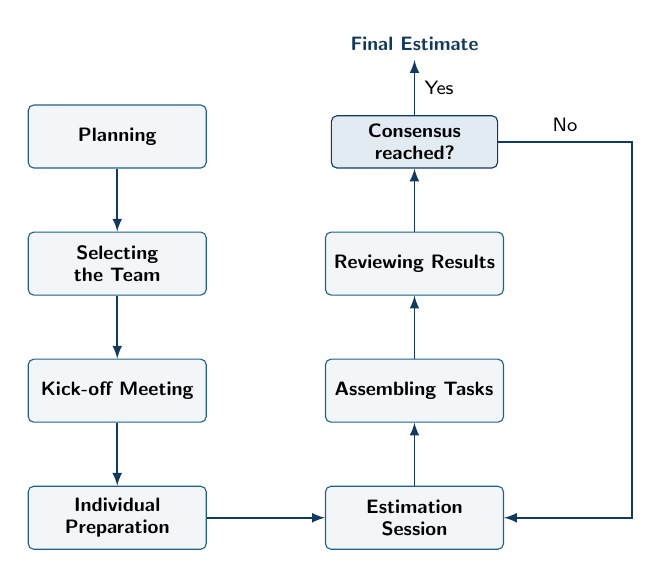
\begin{tikzpicture}[
  node distance=8mm,
  box/.style={draw=uiuBlue,fill=lvl3Row,rounded corners=2pt,align=center,
              font=\sffamily\scriptsize\bfseries,minimum height=8mm,text width=2.05cm,inner sep=3pt},
  dec/.style={draw=uiuNavy,fill=lvl2Row,align=center,font=\sffamily\scriptsize\bfseries,
              inner sep=3pt,text width=1.9cm,rounded corners=2pt},
  ar/.style={-latex,draw=uiuNavy,line width=0.6pt}]
\node[box] (p) {Planning};
\node[box,below=of p] (s) {Selecting the Team};
\node[box,below=of s] (k) {Kick-off Meeting};
\node[box,below=of k] (i) {Individual Preparation};
\node[box,right=15mm of i] (e) {Estimation Session};
\node[box,above=of e] (a) {Assembling Tasks};
\node[box,above=of a] (r) {Reviewing Results};
\node[dec,above=8mm of r] (d) {Consensus reached?};
\node[font=\sffamily\scriptsize\bfseries,text=uiuNavy,above=7mm of d] (end) {Final Estimate};
\draw[ar] (p) -- (s);
\draw[ar] (s) -- (k);
\draw[ar] (k) -- (i);
\draw[ar] (i) -- (e);
\draw[ar] (e) -- (a);
\draw[ar] (a) -- (r);
\draw[ar] (r) -- (d);
\draw[ar] (d) -- node[right,font=\sffamily\scriptsize] {Yes} (end);
\draw[ar] (d.east) -- ++(1.7,0) node[midway,above,font=\sffamily\scriptsize] {No} |- (e.east);
\end{tikzpicture}
\caption{The Wideband Delphi cycle as executed by Team 09}
\label{fig:delphiflow}
\end{figure}

\subsection{Step 1 --- Choosing the Team}

The estimation team should contain three to seven people and should include a
representative of every group that will do the work. Team 09 used five
estimators; the project manager also acted as moderator.


\begin{table}[htbp]
\centering
\caption{The five estimators of the CampusConnect Wideband Delphi session}
\label{tab:experts}
\begin{tabular}{|C{1.1cm}|L{5.0cm}|L{8.0cm}|}
\hline
\rowhead \thead{Ref.} & \thead{Estimator} & \thead{Perspective Represented} \\ \hline
E1 & Sindeed Shuaib Arpon & Moderator / Project Manager --- back-end services \\ \hline
\rowcolor{lvl3Row}
E2 & Nafiz Iqbal Razin & Front-end and UI/UX implementation \\ \hline
E3 & Afnan Zaman Mohammad Sajid & Database design and API integration \\ \hline
\rowcolor{lvl3Row}
E4 & Farzana Akter & Quality assurance, testing and documentation \\ \hline
E5 & Invited Reviewer (senior student) & External domain expert --- built the previous departmental portal \\ \hline
\end{tabular}
\end{table}

The fifth estimator is deliberately external to the team. A group of four people
who have planned the project together tends to share the same blind spots;
inviting a senior student who had already built a departmental portal gave the
session one voice that had not been part of the earlier design discussions, and
that voice produced several of the largest Round~1 deviations.

\subsection{Step 2 --- Kick-off Meeting}

The moderator opened the session by fixing three things that every estimator then
worked to identically.

\begin{keybox}
\textbf{Goal statement.} To estimate the total development effort required to
build UIU CampusConnect, a campus social and academic networking platform, to a
deployable first release.

\medskip
\textbf{Unit of estimation.} Person-days of direct development effort, where one
person-day is eight hours of focused work. Estimates measure \emph{effort}, never
calendar time.

\medskip
\textbf{Task list.} The twelve Level-2 deliverable components of the Work
Breakdown Structure in Chapter~\ref{ch:wbs}, so that every estimate maps directly
onto a WBS code.
\end{keybox}

The meeting also agreed the exclusions: waiting time, holidays and examination
weeks are calendar effects and are not estimated, and project overhead such as
report writing and meetings is tracked separately rather than being distributed
across the tasks.

\subsection{Step 3 --- Individual Preparation}

Each estimator then worked alone, producing an estimate for every task on the
list together with the assumptions behind it. No estimator saw another's figures.
The shared assumptions that emerged from this step are recorded in
Table~\ref{tab:assumptions}; several of them were only written down after Round~1
exposed a disagreement.


\begin{table}[htbp]
\centering
\caption{Assumptions agreed during the estimation session}
\label{tab:assumptions}
\footnotesize
\begin{tabular}{|C{1.3cm}|L{4.6cm}|L{8.0cm}|}
\hline
\rowhead \thead{\footnotesize WBS} & \thead{\footnotesize Task} & \thead{\footnotesize Governing Assumption} \\ \hline
1.1 & System architecture \& UI/UX design & Design system reused across modules; no bespoke iconography. \\ \hline
\rowcolor{lvl3Row}
1.2 & Build, CI/CD pipeline \& integration testing & Free-tier CI runner; single staging environment. \\ \hline
1.3 & Documentation, security audit \& deployment & Penetration testing performed in-house, not outsourced. \\ \hline
\rowcolor{lvl3Row}
2.1 & Authentication \& profile management & University e-mail verification endpoint is available. \\ \hline
2.2 & Direct communication \& alerts & Notification engine built once and reused by all modules. \\ \hline
\rowcolor{lvl3Row}
3.1 & Feed engine \& discovery & Ranking is rule-based; no machine-learning component. \\ \hline
3.2 & Post interactivity \& content control & Media stored on object storage, not on the application server. \\ \hline
\rowcolor{lvl3Row}
4.1 & Notices \& announcements & Section and department lists can be imported, not typed in. \\ \hline
4.2 & Campus events \& attendance (QR check-in) & An open-source QR library is used; only token logic is written. \\ \hline
\rowcolor{lvl3Row}
4.3 & Clubs \& community groups & Club committee data seeded manually for the first release. \\ \hline
5.1 & Peer-to-peer campus services & No payment handling; marketplace is listing-only. \\ \hline
\rowcolor{lvl3Row}
5.2 & Administration \& platform governance & Audit log is append-only in the existing database. \\ \hline
\end{tabular}
\end{table}
\clearpage

\subsection{Step 4 --- The Estimation Form}

Each estimator recorded their work on a standard estimation form. The
\textbf{Est.} column holds the Round~1 figure produced during individual
preparation; \textbf{$\Delta$1} and \textbf{$\Delta$2} record the revisions the
estimator chose to make after the Round~1 and Round~2 discussions; and
\textbf{Total} is the estimator's final Round~3 figure. A blank delta means the
estimator saw no reason to move.

The five completed forms are reproduced below.

\begin{table}[htbp]\centering\footnotesize
\caption{Estimation form --- Sindeed Shuaib Arpon (E1)}
\begin{tabular}{|C{1.1cm}|L{5.0cm}|C{1.1cm}|C{1.0cm}|C{1.0cm}|C{1.1cm}|}
\hline
\rowhead \multicolumn{6}{|L{12.1cm}|}{\thead{\footnotesize Goal: estimate the effort to build UIU CampusConnect to a deployable first release. \quad Units: person-days}} \\ \hline
\rowhead \thead{\footnotesize WBS} & \thead{\footnotesize Task name} & \thead{\footnotesize Est.} & \thead{\footnotesize $\Delta$1} & \thead{\footnotesize $\Delta$2} & \thead{\footnotesize Total} \\ \hline
1.1 & System architecture \& UI/UX design & 6 & $+$1 & $+$1 & \textbf{8} \\ \hline
\rowcolor{lvl3Row}
1.2 & Build, CI/CD pipeline \& integration testing & 4 & $+$1 & $+$1 & \textbf{6} \\ \hline
1.3 & Documentation, security audit \& deployment & 3 & $+$1 & $+$1 & \textbf{5} \\ \hline
\rowcolor{lvl3Row}
2.1 & Authentication \& profile management & 10 & $+$2 & $+$2 & \textbf{14} \\ \hline
2.2 & Direct communication \& alerts & 11 & $+$2 & $+$1 & \textbf{14} \\ \hline
\rowcolor{lvl3Row}
3.1 & Feed engine \& discovery & 8 & $+$1 & $+$2 & \textbf{11} \\ \hline
3.2 & Post interactivity \& content control & 10 & $+$2 & $+$1 & \textbf{13} \\ \hline
\rowcolor{lvl3Row}
4.1 & Notices \& announcements & 7 & $+$1 & $+$2 & \textbf{10} \\ \hline
4.2 & Campus events \& attendance (QR check-in) & 5 & $+$2 & $+$2 & \textbf{9} \\ \hline
\rowcolor{lvl3Row}
4.3 & Clubs \& community groups & 8 & $+$1 & $+$1 & \textbf{10} \\ \hline
5.1 & Peer-to-peer campus services & 9 & $+$1 & $+$2 & \textbf{12} \\ \hline
\rowcolor{lvl3Row}
5.2 & Administration \& platform governance & 9 & $+$2 & $+$2 & \textbf{13} \\ \hline
\rowcolor{lvl1Row}
\multicolumn{2}{|r|}{\textbf{Total (person-days)}} & \textbf{90} & \textbf{$+$17} & \textbf{$+$18} & \textbf{125} \\ \hline
\end{tabular}\end{table}
\begin{table}[htbp]\centering\footnotesize
\caption{Estimation form --- Nafiz Iqbal Razin (E2)}
\begin{tabular}{|C{1.1cm}|L{5.0cm}|C{1.1cm}|C{1.0cm}|C{1.0cm}|C{1.1cm}|}
\hline
\rowhead \multicolumn{6}{|L{12.1cm}|}{\thead{\footnotesize Goal: estimate the effort to build UIU CampusConnect to a deployable first release. \quad Units: person-days}} \\ \hline
\rowhead \thead{\footnotesize WBS} & \thead{\footnotesize Task name} & \thead{\footnotesize Est.} & \thead{\footnotesize $\Delta$1} & \thead{\footnotesize $\Delta$2} & \thead{\footnotesize Total} \\ \hline
1.1 & System architecture \& UI/UX design & 10 & $-$1 & $-$1 & \textbf{8} \\ \hline
\rowcolor{lvl3Row}
1.2 & Build, CI/CD pipeline \& integration testing & 8 & $-$1 & $-$1 & \textbf{6} \\ \hline
1.3 & Documentation, security audit \& deployment & 7 & $-$1 & $-$1 & \textbf{5} \\ \hline
\rowcolor{lvl3Row}
2.1 & Authentication \& profile management & 18 & $-$2 & $-$1 & \textbf{15} \\ \hline
2.2 & Direct communication \& alerts & 17 & $-$2 & $-$1 & \textbf{14} \\ \hline
\rowcolor{lvl3Row}
3.1 & Feed engine \& discovery & 14 & $-$2 & $-$1 & \textbf{11} \\ \hline
3.2 & Post interactivity \& content control & 16 & $-$1 & $-$1 & \textbf{14} \\ \hline
\rowcolor{lvl3Row}
4.1 & Notices \& announcements & 12 & $-$1 & $-$1 & \textbf{10} \\ \hline
4.2 & Campus events \& attendance (QR check-in) & 14 & $-$3 & $-$2 & \textbf{9} \\ \hline
\rowcolor{lvl3Row}
4.3 & Clubs \& community groups & 13 & $-$2 & $-$1 & \textbf{10} \\ \hline
5.1 & Peer-to-peer campus services & 15 & $-$1 & $-$2 & \textbf{12} \\ \hline
\rowcolor{lvl3Row}
5.2 & Administration \& platform governance & 16 & $-$2 & $-$1 & \textbf{13} \\ \hline
\rowcolor{lvl1Row}
\multicolumn{2}{|r|}{\textbf{Total (person-days)}} & \textbf{160} & \textbf{$-$19} & \textbf{$-$14} & \textbf{127} \\ \hline
\end{tabular}\end{table}
\clearpage
\begin{table}[htbp]\centering\footnotesize
\caption{Estimation form --- Afnan Zaman Mohammad Sajid (E3)}
\begin{tabular}{|C{1.1cm}|L{5.0cm}|C{1.1cm}|C{1.0cm}|C{1.0cm}|C{1.1cm}|}
\hline
\rowhead \multicolumn{6}{|L{12.1cm}|}{\thead{\footnotesize Goal: estimate the effort to build UIU CampusConnect to a deployable first release. \quad Units: person-days}} \\ \hline
\rowhead \thead{\footnotesize WBS} & \thead{\footnotesize Task name} & \thead{\footnotesize Est.} & \thead{\footnotesize $\Delta$1} & \thead{\footnotesize $\Delta$2} & \thead{\footnotesize Total} \\ \hline
1.1 & System architecture \& UI/UX design & 7 & $+$1 & $-$1 & \textbf{7} \\ \hline
\rowcolor{lvl3Row}
1.2 & Build, CI/CD pipeline \& integration testing & 5 & $+$1 & $-$1 & \textbf{5} \\ \hline
1.3 & Documentation, security audit \& deployment & 4 & $+$1 & $-$1 & \textbf{4} \\ \hline
\rowcolor{lvl3Row}
2.1 & Authentication \& profile management & 12 & $+$1 &  & \textbf{13} \\ \hline
2.2 & Direct communication \& alerts & 20 & $-$3 & $-$2 & \textbf{15} \\ \hline
\rowcolor{lvl3Row}
3.1 & Feed engine \& discovery & 9 & $+$1 &  & \textbf{10} \\ \hline
3.2 & Post interactivity \& content control & 18 & $-$2 & $-$1 & \textbf{15} \\ \hline
\rowcolor{lvl3Row}
4.1 & Notices \& announcements & 8 & $+$1 &  & \textbf{9} \\ \hline
4.2 & Campus events \& attendance (QR check-in) & 7 & $+$1 &  & \textbf{8} \\ \hline
\rowcolor{lvl3Row}
4.3 & Clubs \& community groups & 9 & $+$1 & $-$1 & \textbf{9} \\ \hline
5.1 & Peer-to-peer campus services & 10 & $+$1 &  & \textbf{11} \\ \hline
\rowcolor{lvl3Row}
5.2 & Administration \& platform governance & 11 & $+$1 &  & \textbf{12} \\ \hline
\rowcolor{lvl1Row}
\multicolumn{2}{|r|}{\textbf{Total (person-days)}} & \textbf{120} & \textbf{$+$5} & \textbf{$-$7} & \textbf{118} \\ \hline
\end{tabular}\end{table}
\begin{table}[htbp]\centering\footnotesize
\caption{Estimation form --- Farzana Akter (E4)}
\begin{tabular}{|C{1.1cm}|L{5.0cm}|C{1.1cm}|C{1.0cm}|C{1.0cm}|C{1.1cm}|}
\hline
\rowhead \multicolumn{6}{|L{12.1cm}|}{\thead{\footnotesize Goal: estimate the effort to build UIU CampusConnect to a deployable first release. \quad Units: person-days}} \\ \hline
\rowhead \thead{\footnotesize WBS} & \thead{\footnotesize Task name} & \thead{\footnotesize Est.} & \thead{\footnotesize $\Delta$1} & \thead{\footnotesize $\Delta$2} & \thead{\footnotesize Total} \\ \hline
1.1 & System architecture \& UI/UX design & 12 & $-$2 & $-$1 & \textbf{9} \\ \hline
\rowcolor{lvl3Row}
1.2 & Build, CI/CD pipeline \& integration testing & 9 & $-$2 &  & \textbf{7} \\ \hline
1.3 & Documentation, security audit \& deployment & 8 & $-$2 &  & \textbf{6} \\ \hline
\rowcolor{lvl3Row}
2.1 & Authentication \& profile management & 20 & $-$3 & $-$2 & \textbf{15} \\ \hline
2.2 & Direct communication \& alerts & 12 & $+$1 &  & \textbf{13} \\ \hline
\rowcolor{lvl3Row}
3.1 & Feed engine \& discovery & 15 & $-$2 & $-$1 & \textbf{12} \\ \hline
3.2 & Post interactivity \& content control & 13 &  & $+$1 & \textbf{14} \\ \hline
\rowcolor{lvl3Row}
4.1 & Notices \& announcements & 14 & $-$2 & $-$1 & \textbf{11} \\ \hline
4.2 & Campus events \& attendance (QR check-in) & 16 & $-$4 & $-$2 & \textbf{10} \\ \hline
\rowcolor{lvl3Row}
4.3 & Clubs \& community groups & 12 & $-$1 &  & \textbf{11} \\ \hline
5.1 & Peer-to-peer campus services & 16 & $-$2 & $-$1 & \textbf{13} \\ \hline
\rowcolor{lvl3Row}
5.2 & Administration \& platform governance & 17 & $-$2 & $-$1 & \textbf{14} \\ \hline
\rowcolor{lvl1Row}
\multicolumn{2}{|r|}{\textbf{Total (person-days)}} & \textbf{164} & \textbf{$-$21} & \textbf{$-$8} & \textbf{135} \\ \hline
\end{tabular}\end{table}
\clearpage
\begin{table}[htbp]\centering\footnotesize
\caption{Estimation form --- Invited Reviewer (senior student) (E5)}
\begin{tabular}{|C{1.1cm}|L{5.0cm}|C{1.1cm}|C{1.0cm}|C{1.0cm}|C{1.1cm}|}
\hline
\rowhead \multicolumn{6}{|L{12.1cm}|}{\thead{\footnotesize Goal: estimate the effort to build UIU CampusConnect to a deployable first release. \quad Units: person-days}} \\ \hline
\rowhead \thead{\footnotesize WBS} & \thead{\footnotesize Task name} & \thead{\footnotesize Est.} & \thead{\footnotesize $\Delta$1} & \thead{\footnotesize $\Delta$2} & \thead{\footnotesize Total} \\ \hline
1.1 & System architecture \& UI/UX design & 9 & $-$1 &  & \textbf{8} \\ \hline
\rowcolor{lvl3Row}
1.2 & Build, CI/CD pipeline \& integration testing & 6 &  &  & \textbf{6} \\ \hline
1.3 & Documentation, security audit \& deployment & 5 &  &  & \textbf{5} \\ \hline
\rowcolor{lvl3Row}
2.1 & Authentication \& profile management & 15 & $-$1 & $-$1 & \textbf{13} \\ \hline
2.2 & Direct communication \& alerts & 14 &  &  & \textbf{14} \\ \hline
\rowcolor{lvl3Row}
3.1 & Feed engine \& discovery & 12 & $-$1 &  & \textbf{11} \\ \hline
3.2 & Post interactivity \& content control & 15 & $-$1 &  & \textbf{14} \\ \hline
\rowcolor{lvl3Row}
4.1 & Notices \& announcements & 10 &  &  & \textbf{10} \\ \hline
4.2 & Campus events \& attendance (QR check-in) & 10 & $-$1 &  & \textbf{9} \\ \hline
\rowcolor{lvl3Row}
4.3 & Clubs \& community groups & 11 & $-$1 &  & \textbf{10} \\ \hline
5.1 & Peer-to-peer campus services & 13 & $-$1 &  & \textbf{12} \\ \hline
\rowcolor{lvl3Row}
5.2 & Administration \& platform governance & 14 & $-$1 &  & \textbf{13} \\ \hline
\rowcolor{lvl1Row}
\multicolumn{2}{|r|}{\textbf{Total (person-days)}} & \textbf{134} & \textbf{$-$8} & \textbf{$-$1} & \textbf{125} \\ \hline
\end{tabular}\end{table}
\clearpage

\section{Estimation Session: Three Rounds}

The moderator collected the forms, plotted the totals anonymously and led the
discussion. Three rounds were required before the group agreed that the range was
acceptable. The tables below give every estimator's figure for every task in each
round, together with the spread.

\subsection{Round 1 --- Independent Estimates}

Round~1 is the output of individual preparation: five people estimating the same
twelve components with no discussion between them. The spread is correspondingly
wide.

\begin{table}[htbp]\centering\footnotesize
\caption{Round 1 --- independent estimates from individual preparation (person-days)}
\label{tab:round1}
\begin{tabular}{|C{1.05cm}|L{4.35cm}|C{0.85cm}|C{0.85cm}|C{0.85cm}|C{0.85cm}|C{0.85cm}|C{0.9cm}|C{0.9cm}|C{0.9cm}|}
\hline
\rowhead \thead{\footnotesize WBS} & \thead{\footnotesize Task} & \thead{\footnotesize E1} & \thead{\footnotesize E2} & \thead{\footnotesize E3} & \thead{\footnotesize E4} & \thead{\footnotesize E5} & \thead{\footnotesize Min} & \thead{\footnotesize Max} & \thead{\footnotesize Mean} \\ \hline
1.1 & System architecture \& UI/UX design & 6 & 10 & 7 & 12 & 9 & 6 & 12 & 8.8 \\ \hline
\rowcolor{lvl3Row}
1.2 & Build, CI/CD pipeline \& integration testing & 4 & 8 & 5 & 9 & 6 & 4 & 9 & 6.4 \\ \hline
1.3 & Documentation, security audit \& deployment & 3 & 7 & 4 & 8 & 5 & 3 & 8 & 5.4 \\ \hline
\rowcolor{lvl3Row}
2.1 & Authentication \& profile management & 10 & 18 & 12 & 20 & 15 & 10 & 20 & 15 \\ \hline
2.2 & Direct communication \& alerts & 11 & 17 & 20 & 12 & 14 & 11 & 20 & 14.8 \\ \hline
\rowcolor{lvl3Row}
3.1 & Feed engine \& discovery & 8 & 14 & 9 & 15 & 12 & 8 & 15 & 11.6 \\ \hline
3.2 & Post interactivity \& content control & 10 & 16 & 18 & 13 & 15 & 10 & 18 & 14.4 \\ \hline
\rowcolor{lvl3Row}
4.1 & Notices \& announcements & 7 & 12 & 8 & 14 & 10 & 7 & 14 & 10.2 \\ \hline
4.2 & Campus events \& attendance (QR check-in) & 5 & 14 & 7 & 16 & 10 & 5 & 16 & 10.4 \\ \hline
\rowcolor{lvl3Row}
4.3 & Clubs \& community groups & 8 & 13 & 9 & 12 & 11 & 8 & 13 & 10.6 \\ \hline
5.1 & Peer-to-peer campus services & 9 & 15 & 10 & 16 & 13 & 9 & 16 & 12.6 \\ \hline
\rowcolor{lvl3Row}
5.2 & Administration \& platform governance & 9 & 16 & 11 & 17 & 14 & 9 & 17 & 13.4 \\ \hline
\rowcolor{lvl1Row}
\multicolumn{2}{|r|}{\textbf{Total}} & \textbf{90} & \textbf{160} & \textbf{120} & \textbf{164} & \textbf{134} & \textbf{90} & \textbf{164} & \textbf{133.6} \\ \hline
\end{tabular}\end{table}

The project totals ranged from 90 to 164 person-days --- a spread of
74 days, or 55\% of the mean. That is far too wide to plan
against, but the pattern of the disagreement was informative: E1 and E3 were
consistently low and E2 and E4 consistently high, which suggested a systematic
difference in what ``done'' meant rather than random noise. The discussion
confirmed it --- the low estimators had assumed that testing and documentation
were counted in task 1.3, while the high estimators had included per-module
testing inside every task.

\subsection{Round 2 --- After the First Assumption Review}

With the testing boundary settled and the assumptions of
Table~\ref{tab:assumptions} written down, every estimator re-estimated. Note that
the moderator showed only the anonymous distribution, never who gave which
number.

\begin{table}[htbp]\centering\footnotesize
\caption{Round 2 --- estimates after the first assumption review (person-days)}
\label{tab:round2}
\begin{tabular}{|C{1.05cm}|L{4.35cm}|C{0.85cm}|C{0.85cm}|C{0.85cm}|C{0.85cm}|C{0.85cm}|C{0.9cm}|C{0.9cm}|C{0.9cm}|}
\hline
\rowhead \thead{\footnotesize WBS} & \thead{\footnotesize Task} & \thead{\footnotesize E1} & \thead{\footnotesize E2} & \thead{\footnotesize E3} & \thead{\footnotesize E4} & \thead{\footnotesize E5} & \thead{\footnotesize Min} & \thead{\footnotesize Max} & \thead{\footnotesize Mean} \\ \hline
1.1 & System architecture \& UI/UX design & 7 & 9 & 8 & 10 & 8 & 7 & 10 & 8.4 \\ \hline
\rowcolor{lvl3Row}
1.2 & Build, CI/CD pipeline \& integration testing & 5 & 7 & 6 & 7 & 6 & 5 & 7 & 6.2 \\ \hline
1.3 & Documentation, security audit \& deployment & 4 & 6 & 5 & 6 & 5 & 4 & 6 & 5.2 \\ \hline
\rowcolor{lvl3Row}
2.1 & Authentication \& profile management & 12 & 16 & 13 & 17 & 14 & 12 & 17 & 14.4 \\ \hline
2.2 & Direct communication \& alerts & 13 & 15 & 17 & 13 & 14 & 13 & 17 & 14.4 \\ \hline
\rowcolor{lvl3Row}
3.1 & Feed engine \& discovery & 9 & 12 & 10 & 13 & 11 & 9 & 13 & 11 \\ \hline
3.2 & Post interactivity \& content control & 12 & 15 & 16 & 13 & 14 & 12 & 16 & 14 \\ \hline
\rowcolor{lvl3Row}
4.1 & Notices \& announcements & 8 & 11 & 9 & 12 & 10 & 8 & 12 & 10 \\ \hline
4.2 & Campus events \& attendance (QR check-in) & 7 & 11 & 8 & 12 & 9 & 7 & 12 & 9.4 \\ \hline
\rowcolor{lvl3Row}
4.3 & Clubs \& community groups & 9 & 11 & 10 & 11 & 10 & 9 & 11 & 10.2 \\ \hline
5.1 & Peer-to-peer campus services & 10 & 14 & 11 & 14 & 12 & 10 & 14 & 12.2 \\ \hline
\rowcolor{lvl3Row}
5.2 & Administration \& platform governance & 11 & 14 & 12 & 15 & 13 & 11 & 15 & 13 \\ \hline
\rowcolor{lvl1Row}
\multicolumn{2}{|r|}{\textbf{Total}} & \textbf{107} & \textbf{141} & \textbf{125} & \textbf{143} & \textbf{126} & \textbf{107} & \textbf{143} & \textbf{128.4} \\ \hline
\end{tabular}\end{table}

The spread narrowed from 74 to 36 person-days. Two tasks remained
contentious: 2.2 (direct communication and alerts), where E3 still estimated
real-time messaging well above the group, and 4.2 (campus events and attendance),
which is examined in detail in Section~\ref{sec:convergence}.

\subsection{Round 3 --- Convergence}

The third round resolved the two remaining disagreements. E3's messaging estimate
was accepted as partly justified --- the group raised its own figures for 2.2
rather than E3 lowering theirs --- and the QR check-in assumption was settled.

\begin{table}[htbp]\centering\footnotesize
\caption{Round 3 --- converged estimates accepted as the project baseline (person-days)}
\label{tab:round3}
\begin{tabular}{|C{1.05cm}|L{4.35cm}|C{0.85cm}|C{0.85cm}|C{0.85cm}|C{0.85cm}|C{0.85cm}|C{0.9cm}|C{0.9cm}|C{0.9cm}|}
\hline
\rowhead \thead{\footnotesize WBS} & \thead{\footnotesize Task} & \thead{\footnotesize E1} & \thead{\footnotesize E2} & \thead{\footnotesize E3} & \thead{\footnotesize E4} & \thead{\footnotesize E5} & \thead{\footnotesize Min} & \thead{\footnotesize Max} & \thead{\footnotesize Mean} \\ \hline
1.1 & System architecture \& UI/UX design & 8 & 8 & 7 & 9 & 8 & 7 & 9 & 8 \\ \hline
\rowcolor{lvl3Row}
1.2 & Build, CI/CD pipeline \& integration testing & 6 & 6 & 5 & 7 & 6 & 5 & 7 & 6 \\ \hline
1.3 & Documentation, security audit \& deployment & 5 & 5 & 4 & 6 & 5 & 4 & 6 & 5 \\ \hline
\rowcolor{lvl3Row}
2.1 & Authentication \& profile management & 14 & 15 & 13 & 15 & 13 & 13 & 15 & 14 \\ \hline
2.2 & Direct communication \& alerts & 14 & 14 & 15 & 13 & 14 & 13 & 15 & 14 \\ \hline
\rowcolor{lvl3Row}
3.1 & Feed engine \& discovery & 11 & 11 & 10 & 12 & 11 & 10 & 12 & 11 \\ \hline
3.2 & Post interactivity \& content control & 13 & 14 & 15 & 14 & 14 & 13 & 15 & 14 \\ \hline
\rowcolor{lvl3Row}
4.1 & Notices \& announcements & 10 & 10 & 9 & 11 & 10 & 9 & 11 & 10 \\ \hline
4.2 & Campus events \& attendance (QR check-in) & 9 & 9 & 8 & 10 & 9 & 8 & 10 & 9 \\ \hline
\rowcolor{lvl3Row}
4.3 & Clubs \& community groups & 10 & 10 & 9 & 11 & 10 & 9 & 11 & 10 \\ \hline
5.1 & Peer-to-peer campus services & 12 & 12 & 11 & 13 & 12 & 11 & 13 & 12 \\ \hline
\rowcolor{lvl3Row}
5.2 & Administration \& platform governance & 13 & 13 & 12 & 14 & 13 & 12 & 14 & 13 \\ \hline
\rowcolor{lvl1Row}
\multicolumn{2}{|r|}{\textbf{Total}} & \textbf{125} & \textbf{127} & \textbf{118} & \textbf{135} & \textbf{125} & \textbf{118} & \textbf{135} & \textbf{126} \\ \hline
\end{tabular}\end{table}

At this point no estimator wished to move further and the group agreed that the
remaining range of 17 person-days (13\% of the mean)
was acceptable for planning. Round~3 is therefore the accepted baseline.


\section{Convergence Analysis}
\label{sec:convergence}

Table~\ref{tab:convergence} summarises how the project total behaved across the
three rounds, and Figure~\ref{fig:convtotal} plots the same data in the form the
moderator drew on the whiteboard at the start of each round.


\begin{table}[htbp]
\centering
\caption{Convergence of the project total across three rounds}
\label{tab:convergence}
\begin{tabular}{|C{1.8cm}|C{1.8cm}|C{1.8cm}|C{1.8cm}|C{2.4cm}|C{3.0cm}|}
\hline
\rowhead \thead{Round} & \thead{Minimum} & \thead{Maximum} & \thead{Range} & \thead{Mean} & \thead{Spread (\% of mean)} \\ \hline
Round 1 & 90 & 164 & 74 & 133.6 & 55.4\% \\ \hline
\rowcolor{lvl3Row}
Round 2 & 107 & 143 & 36 & 128.4 & 28.0\% \\ \hline
Round 3 & 118 & 135 & 17 & 126 & 13.5\% \\ \hline
\end{tabular}
\end{table}

\begin{figure}[htbp]
\centering
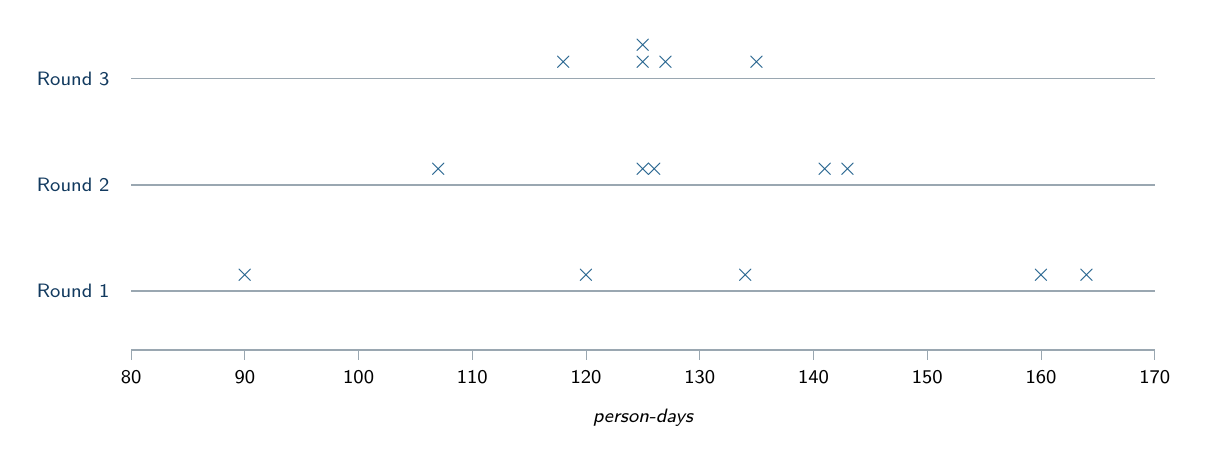
\begin{tikzpicture}[x=1cm,y=1cm]
\draw[lineGrey,line width=0.6pt] (0,0.0) -- (13.00,0.0);
\node[anchor=east,font=\sffamily\scriptsize,text=uiuNavy] at (-0.15,0.0) {Round 1};
\node[font=\bfseries\small,text=uiuBlue] at (1.444,0.20) {$\times$};
\node[font=\bfseries\small,text=uiuBlue] at (11.556,0.20) {$\times$};
\node[font=\bfseries\small,text=uiuBlue] at (5.778,0.20) {$\times$};
\node[font=\bfseries\small,text=uiuBlue] at (12.133,0.20) {$\times$};
\node[font=\bfseries\small,text=uiuBlue] at (7.8,0.20) {$\times$};
\draw[lineGrey,line width=0.6pt] (0,1.35) -- (13.00,1.35);
\node[anchor=east,font=\sffamily\scriptsize,text=uiuNavy] at (-0.15,1.35) {Round 2};
\node[font=\bfseries\small,text=uiuBlue] at (3.9,1.55) {$\times$};
\node[font=\bfseries\small,text=uiuBlue] at (8.811,1.55) {$\times$};
\node[font=\bfseries\small,text=uiuBlue] at (6.5,1.55) {$\times$};
\node[font=\bfseries\small,text=uiuBlue] at (9.1,1.55) {$\times$};
\node[font=\bfseries\small,text=uiuBlue] at (6.644,1.55) {$\times$};
\draw[lineGrey,line width=0.6pt] (0,2.7) -- (13.00,2.7);
\node[anchor=east,font=\sffamily\scriptsize,text=uiuNavy] at (-0.15,2.7) {Round 3};
\node[font=\bfseries\small,text=uiuBlue] at (6.5,2.90) {$\times$};
\node[font=\bfseries\small,text=uiuBlue] at (6.789,2.90) {$\times$};
\node[font=\bfseries\small,text=uiuBlue] at (5.489,2.90) {$\times$};
\node[font=\bfseries\small,text=uiuBlue] at (7.944,2.90) {$\times$};
\node[font=\bfseries\small,text=uiuBlue] at (6.5,3.12) {$\times$};
\draw[lineGrey,line width=0.6pt] (0,-0.75) -- (13.00,-0.75);
\draw[lineGrey] (0.000,-0.75) -- (0.000,-0.87);
\node[font=\sffamily\scriptsize,anchor=north] at (0.000,-0.89) {80};
\draw[lineGrey] (1.444,-0.75) -- (1.444,-0.87);
\node[font=\sffamily\scriptsize,anchor=north] at (1.444,-0.89) {90};
\draw[lineGrey] (2.889,-0.75) -- (2.889,-0.87);
\node[font=\sffamily\scriptsize,anchor=north] at (2.889,-0.89) {100};
\draw[lineGrey] (4.333,-0.75) -- (4.333,-0.87);
\node[font=\sffamily\scriptsize,anchor=north] at (4.333,-0.89) {110};
\draw[lineGrey] (5.778,-0.75) -- (5.778,-0.87);
\node[font=\sffamily\scriptsize,anchor=north] at (5.778,-0.89) {120};
\draw[lineGrey] (7.222,-0.75) -- (7.222,-0.87);
\node[font=\sffamily\scriptsize,anchor=north] at (7.222,-0.89) {130};
\draw[lineGrey] (8.667,-0.75) -- (8.667,-0.87);
\node[font=\sffamily\scriptsize,anchor=north] at (8.667,-0.89) {140};
\draw[lineGrey] (10.111,-0.75) -- (10.111,-0.87);
\node[font=\sffamily\scriptsize,anchor=north] at (10.111,-0.89) {150};
\draw[lineGrey] (11.556,-0.75) -- (11.556,-0.87);
\node[font=\sffamily\scriptsize,anchor=north] at (11.556,-0.89) {160};
\draw[lineGrey] (13.000,-0.75) -- (13.000,-0.87);
\node[font=\sffamily\scriptsize,anchor=north] at (13.000,-0.89) {170};
\node[font=\sffamily\scriptsize\itshape,anchor=north] at (6.50,-1.37) {person-days};
\end{tikzpicture}
\caption{Whiteboard plot of the project totals. Each $\times$ is one estimator; the
distribution tightens with every round.}
\label{fig:convtotal}
\end{figure}

The range fell from 74 person-days to 36 and then to 17, while the mean moved only from 133.6 to 126 person-days.
That combination --- a collapsing range around a stable centre --- is the signature
of a healthy Delphi session. A mean that drifts steadily in one direction instead
would indicate that the group was being anchored rather than reaching agreement.


\section{Feature-Level Convergence: 4.2 Campus Events \& Attendance}

The project total hides the most instructive part of the session. Task~4.2 ---
event publishing, registration and QR/token check-in --- produced the widest
disagreement of Round~1 and is worked through here in full, because it shows what
the technique is actually for.

\begin{table}[htbp]\centering
\caption{Three-round estimation of WBS 4.2 --- Campus Events \& Attendance (person-days)}
\label{tab:feature42}
\begin{tabular}{|L{1.9cm}|C{1.0cm}|C{1.0cm}|C{1.0cm}|C{1.0cm}|C{1.0cm}|C{1.1cm}|C{1.1cm}|C{1.2cm}|C{1.2cm}|}
\hline
\rowhead \thead{Round} & \thead{E1} & \thead{E2} & \thead{E3} & \thead{E4} & \thead{E5} & \thead{Min} & \thead{Max} & \thead{Range} & \thead{Mean} \\ \hline
Round 1 & 5 & 14 & 7 & 16 & 10 & 5 & 16 & 11 & 10.4 \\ \hline
\rowcolor{lvl3Row}
Round 2 & 7 & 11 & 8 & 12 & 9 & 7 & 12 & 5 & 9.4 \\ \hline
Round 3 & 9 & 9 & 8 & 10 & 9 & 8 & 10 & 2 & 9 \\ \hline
\end{tabular}\end{table}
\begin{figure}[htbp]
\centering
\begin{tikzpicture}[x=1cm,y=1cm]
\draw[lineGrey,line width=0.6pt] (0,0.0) -- (12.00,0.0);
\node[anchor=east,font=\sffamily\scriptsize,text=uiuNavy] at (-0.15,0.0) {Round 1};
\node[font=\bfseries\small,text=uiuBlue] at (0.857,0.20) {$\times$};
\node[font=\bfseries\small,text=uiuBlue] at (8.571,0.20) {$\times$};
\node[font=\bfseries\small,text=uiuBlue] at (2.571,0.20) {$\times$};
\node[font=\bfseries\small,text=uiuBlue] at (10.286,0.20) {$\times$};
\node[font=\bfseries\small,text=uiuBlue] at (5.143,0.20) {$\times$};
\draw[lineGrey,line width=0.6pt] (0,1.35) -- (12.00,1.35);
\node[anchor=east,font=\sffamily\scriptsize,text=uiuNavy] at (-0.15,1.35) {Round 2};
\node[font=\bfseries\small,text=uiuBlue] at (2.571,1.55) {$\times$};
\node[font=\bfseries\small,text=uiuBlue] at (6.0,1.55) {$\times$};
\node[font=\bfseries\small,text=uiuBlue] at (3.429,1.55) {$\times$};
\node[font=\bfseries\small,text=uiuBlue] at (6.857,1.55) {$\times$};
\node[font=\bfseries\small,text=uiuBlue] at (4.286,1.55) {$\times$};
\draw[lineGrey,line width=0.6pt] (0,2.7) -- (12.00,2.7);
\node[anchor=east,font=\sffamily\scriptsize,text=uiuNavy] at (-0.15,2.7) {Round 3};
\node[font=\bfseries\small,text=uiuBlue] at (4.286,2.90) {$\times$};
\node[font=\bfseries\small,text=uiuBlue] at (4.286,3.12) {$\times$};
\node[font=\bfseries\small,text=uiuBlue] at (3.429,2.90) {$\times$};
\node[font=\bfseries\small,text=uiuBlue] at (5.143,2.90) {$\times$};
\node[font=\bfseries\small,text=uiuBlue] at (4.286,3.34) {$\times$};
\draw[lineGrey,line width=0.6pt] (0,-0.75) -- (12.00,-0.75);
\draw[lineGrey] (0.000,-0.75) -- (0.000,-0.87);
\node[font=\sffamily\scriptsize,anchor=north] at (0.000,-0.89) {4};
\draw[lineGrey] (1.714,-0.75) -- (1.714,-0.87);
\node[font=\sffamily\scriptsize,anchor=north] at (1.714,-0.89) {6};
\draw[lineGrey] (3.429,-0.75) -- (3.429,-0.87);
\node[font=\sffamily\scriptsize,anchor=north] at (3.429,-0.89) {8};
\draw[lineGrey] (5.143,-0.75) -- (5.143,-0.87);
\node[font=\sffamily\scriptsize,anchor=north] at (5.143,-0.89) {10};
\draw[lineGrey] (6.857,-0.75) -- (6.857,-0.87);
\node[font=\sffamily\scriptsize,anchor=north] at (6.857,-0.89) {12};
\draw[lineGrey] (8.571,-0.75) -- (8.571,-0.87);
\node[font=\sffamily\scriptsize,anchor=north] at (8.571,-0.89) {14};
\draw[lineGrey] (10.286,-0.75) -- (10.286,-0.87);
\node[font=\sffamily\scriptsize,anchor=north] at (10.286,-0.89) {16};
\draw[lineGrey] (12.000,-0.75) -- (12.000,-0.87);
\node[font=\sffamily\scriptsize,anchor=north] at (12.000,-0.89) {18};
\node[font=\sffamily\scriptsize\itshape,anchor=north] at (6.00,-1.37) {person-days};
\end{tikzpicture}
\caption{Estimation-session convergence for WBS 4.2, Campus Events \& Attendance}
\label{fig:conv42}
\end{figure}

\subsection*{What happened in each round}

\textbf{Round 1 --- range 11 days (5 to 16).} The two extremes were not
carelessness; they were two different projects. E1, estimating 5 days, assumed
that an open-source QR library would handle generation and scanning, leaving only
the registration records and a token field to write. E4, estimating 16 days,
assumed the team would implement token generation, signing and scan validation
itself, and had also included the post-event gallery and organiser reporting in
the same task. Neither assumption was written down before the session.

\medskip
\textbf{Round 2 --- range 5 days (7 to 12).} The moderator recorded the agreed
assumption --- \emph{an open-source QR library is used; only the token issue and
validation logic is written} --- and confirmed with reference to the WBS that
4.2.1.3 (post-event gallery) is a separate work package inside the same
component, so it must be counted, but only once. Both extremes moved
substantially: E1 rose because the gallery was now inside the boundary, E4 fell
because the library was now assumed. The remaining gap was about capacity and
waitlist handling, which E2 and E4 considered more intricate than the others.

\medskip
\textbf{Round 3 --- range 2 days (8 to 10).} The waitlist question was resolved by
agreeing that promotion from the waitlist is automatic and requires no
administrator screen. With that settled, all five estimates fell within two days
of each other and the group accepted a consensus of 9 person-days.

\begin{keybox}
\textbf{Why this matters.} The disagreement was never really about effort; it was
about an unwritten assumption. The Delphi session surfaced it in the second week
of planning, at the cost of about twenty minutes of discussion. Had it survived
until Sprint~5, one member would have started writing a QR token library while
another expected the module to be nearly complete --- a rework cost of several
days, and precisely the kind of silent divergence recorded as risk R8 in
Chapter~\ref{ch:risk}.
\end{keybox}


\section{Assembling the Tasks}

After Round~3 the moderator compiled the master estimate. Following standard
practice the sheet records a best case (the sum of the lowest Round-3 estimate for
each task), a worst case (the sum of the highest), and the expected value (the
sum of the means), so that the plan carries its own uncertainty rather than
pretending to a single number.

\begin{table}[htbp]\centering\footnotesize
\caption{Master estimate compiled from Round 3 (person-days)}
\label{tab:master}
\begin{tabular}{|C{1.2cm}|L{5.6cm}|C{1.7cm}|C{1.7cm}|C{1.9cm}|C{1.9cm}|}
\hline
\rowhead \thead{\footnotesize WBS} & \thead{\footnotesize Task} & \thead{\footnotesize Best case} & \thead{\footnotesize Worst case} & \thead{\footnotesize Expected} & \thead{\footnotesize Expected (hours)} \\ \hline
1.1 & System architecture \& UI/UX design & 7 & 9 & 8 & 64 \\ \hline
\rowcolor{lvl3Row}
1.2 & Build, CI/CD pipeline \& integration testing & 5 & 7 & 6 & 48 \\ \hline
1.3 & Documentation, security audit \& deployment & 4 & 6 & 5 & 40 \\ \hline
\rowcolor{lvl3Row}
2.1 & Authentication \& profile management & 13 & 15 & 14 & 112 \\ \hline
2.2 & Direct communication \& alerts & 13 & 15 & 14 & 112 \\ \hline
\rowcolor{lvl3Row}
3.1 & Feed engine \& discovery & 10 & 12 & 11 & 88 \\ \hline
3.2 & Post interactivity \& content control & 13 & 15 & 14 & 112 \\ \hline
\rowcolor{lvl3Row}
4.1 & Notices \& announcements & 9 & 11 & 10 & 80 \\ \hline
4.2 & Campus events \& attendance (QR check-in) & 8 & 10 & 9 & 72 \\ \hline
\rowcolor{lvl3Row}
4.3 & Clubs \& community groups & 9 & 11 & 10 & 80 \\ \hline
5.1 & Peer-to-peer campus services & 11 & 13 & 12 & 96 \\ \hline
\rowcolor{lvl3Row}
5.2 & Administration \& platform governance & 12 & 14 & 13 & 104 \\ \hline
\rowcolor{lvl1Row}
\multicolumn{2}{|r|}{\textbf{Project total}} & \textbf{114} & \textbf{138} & \textbf{126} & \textbf{1008} \\ \hline
\end{tabular}\end{table}

The consensus estimate is therefore \textbf{126 person-days}, or
approximately \textbf{1008 person-hours}, with a planning band of
114 to 138 person-days. Distributed across four team members this is about
31.5 working days each, which fits a single semester provided the sprint
roadmap of Section~\ref{sec:roadmap} is followed and the out-of-scope list of
Chapter~\ref{ch:vision} is enforced.


\section{Reviewing the Results}

The final step is the review meeting, in which the compiled estimate is checked
against what the team already believed. Because the WBS allocated effort as
percentages and the Delphi session produced absolute days, the two can be
compared directly --- and disagreement between them would mean that one of the two
is wrong.

\begin{table}[htbp]\centering
\caption{Cross-check: Delphi consensus against the WBS effort allocation}
\label{tab:crosscheck}
\begin{tabular}{|C{1.4cm}|L{5.8cm}|C{2.2cm}|C{2.2cm}|C{2.0cm}|}
\hline
\rowhead \thead{WBS} & \thead{Task} & \thead{Delphi (days)} & \thead{Delphi share} & \thead{WBS share} \\ \hline
1.1 & System architecture \& UI/UX design & 8 & 6.3\% & 6\% \\ \hline
\rowcolor{lvl3Row}
1.2 & Build, CI/CD pipeline \& integration testing & 6 & 4.8\% & 5\% \\ \hline
1.3 & Documentation, security audit \& deployment & 5 & 4.0\% & 4\% \\ \hline
\rowcolor{lvl3Row}
2.1 & Authentication \& profile management & 14 & 11.1\% & 11\% \\ \hline
2.2 & Direct communication \& alerts & 14 & 11.1\% & 11\% \\ \hline
\rowcolor{lvl3Row}
3.1 & Feed engine \& discovery & 11 & 8.7\% & 9\% \\ \hline
3.2 & Post interactivity \& content control & 14 & 11.1\% & 11\% \\ \hline
\rowcolor{lvl3Row}
4.1 & Notices \& announcements & 10 & 7.9\% & 8\% \\ \hline
4.2 & Campus events \& attendance (QR check-in) & 9 & 7.1\% & 7\% \\ \hline
\rowcolor{lvl3Row}
4.3 & Clubs \& community groups & 10 & 7.9\% & 8\% \\ \hline
5.1 & Peer-to-peer campus services & 12 & 9.5\% & 10\% \\ \hline
\rowcolor{lvl3Row}
5.2 & Administration \& platform governance & 13 & 10.3\% & 10\% \\ \hline
\rowcolor{lvl1Row}
\multicolumn{2}{|r|}{\textbf{Total}} & \textbf{126} & \textbf{100.0\%} & \textbf{100\%} \\ \hline
\end{tabular}\end{table}

No component deviates from its WBS allocation by more than
0.5~percentage points. The two estimates were produced by different
methods --- one by top-down proportional allocation during decomposition, the
other by bottom-up expert consensus --- so their agreement is meaningful
corroboration rather than a tautology. The Delphi result is accepted as the
effort baseline for the project, and it feeds directly into three later decisions:

\begin{itemize}
  \item \textbf{Sprint sizing.} With 126 person-days across seven sprints, a
  sprint carries roughly 18 person-days of work, which is the capacity check
  applied at every sprint planning session in Chapter~\ref{ch:method}.
  \item \textbf{The 40-hour rule.} 1008 person-hours spread over 67 Level-4
  work packages averages about 15 hours per package, confirming that the
  decomposition in Chapter~\ref{ch:wbs} reached the intended 8--40 hour
  granularity.
  \item \textbf{Schedule risk.} The gap between the best case (114 days) and
  the worst case (138 days) is 24 person-days, roughly 19\% of the
  baseline. That figure is the quantitative basis for the schedule contingency
  held against risk R9 in Chapter~\ref{ch:risk}.
\end{itemize}

\section{Limitations of the Estimate}

Two honest qualifications belong with any Delphi result. First, consensus is not
correctness: five people can agree and still be wrong together, particularly when
four of them share the same limited experience --- which is exactly why an
external estimator was invited. Second, the estimate is only as good as its
assumptions, so it is valid only while Table~\ref{tab:assumptions} holds. If the
university e-mail verification endpoint turns out to be unavailable, or if payment
handling is added to the marketplace, the affected tasks must be re-estimated
rather than absorbed silently. The baseline is therefore re-reviewed at every
sprint retrospective against the effort actually recorded.

% ============================================================
\chapter{Risk Management and RMMM}
\label{ch:risk}
% ============================================================

\section{The Concept of Risk in this Project}

A risk is not a problem yet; it is a possibility of a future problem. Risk
analysis and management are the actions a software team takes to understand and
control that uncertainty before it becomes damage. For CampusConnect the
distinction matters practically: the platform stores personal data for the
entire student body, carries official university communication and will face its
heaviest load precisely on the days that matter most -- registration, section
selection and result publication. Discovering these problems in production would
be far more expensive than planning for them now.

Every risk in this project is characterised by two quantities, each scored from
0 to 5:

\begin{itemize}
  \item \textbf{Probability} -- how likely the risk is to occur during the
  project or in early operation.
  \item \textbf{Impact} -- the severity of the consequence for users, data or
  the schedule if it does occur.
\end{itemize}

Their product is the \textbf{risk exposure}, and it is the number the team uses
to decide where to spend limited effort. Exposure of 20 or above is treated as
critical and must have an active mitigation in the current sprint; 10--19 is
significant and is scheduled; below 10 is monitored.

\section{Risk Categories in UIU CampusConnect}

\begin{table}[htbp]
\centering
\caption{Risk categories and concrete CampusConnect examples}
\label{tab:riskcat}
\begin{tabular}{|L{2.7cm}|L{4.0cm}|L{7.7cm}|}
\hline
\rowhead \thead{Category} & \thead{Definition} & \thead{Examples in CampusConnect} \\ \hline
\textbf{Technical risk} &
Arising from technology, tools and system design. &
The notification service fails to deliver under load; a module's API contract
changes and breaks its consumers; the server goes down when the whole batch
opens the results notice at once. \\ \hline
\rowcolor{lvl3Row}
\textbf{Project risk} &
Arising from planning, scheduling and resource allocation. &
A four-member team loses a member to illness mid-sprint; the semester deadline
leaves no slack; the backlog keeps growing as reviewers request new features. \\ \hline
\textbf{Business risk} &
Threatening the value and adoption of the product. &
Students continue to use existing Facebook groups and never adopt the platform;
the university declines to endorse the official notice board, removing its
authority. \\ \hline
\rowcolor{lvl3Row}
\textbf{External risk} &
Originating outside the team's control. &
A change in data-protection expectations forces rework of how personal data is
stored; hosting provider outage; campus closure disrupting user testing. \\ \hline
\end{tabular}
\end{table}

\section{The RMMM Strategy for UIU CampusConnect}

RMMM -- Risk Mitigation, Monitoring and Management -- is the structured plan
through which the team handles risk across the project lifecycle. Rather than
restating the theory, this section describes the procedure the CampusConnect
team actually follows.

\subsection{Risk Mitigation: acting before the risk occurs}

Mitigation is the set of actions taken in advance to reduce either the
probability or the impact of a risk. In this project mitigation is not a
separate phase; it is embedded in the sprint cycle.

\begin{enumerate}
  \item \textbf{Identification.} At every sprint planning session the team asks
  what could go wrong with the work packages selected for that sprint. Anything
  raised is written into the risk register with an owner.
  \item \textbf{Analysis.} Each risk is scored for probability and impact on the
  0--5 scale and its exposure computed. This is what produces the risk plan
  sheet in Section~\ref{sec:riskplan}.
  \item \textbf{Preventive design.} Risks with exposure of 20 or above generate
  concrete engineering work packages in the WBS. Data-privacy risk is why
  encryption and access-control auditing exist as WBS 1.3.1.1; peak-load risk is
  why load testing exists as WBS 1.2.2.2; integration risk is why the automated
  API test suite exists as WBS 1.2.2.1. Mitigation is therefore funded and
  scheduled, not merely intended.
  \item \textbf{Assignment.} Every risk has exactly one named owner among the
  four team members, who is responsible for reporting its status.
\end{enumerate}

\subsection{Risk Monitoring: watching while the project runs}

Monitoring is the continuous process of tracking known risks and detecting new
ones. The team's monitoring mechanisms are deliberately lightweight so that they
are actually performed.

\begin{itemize}
  \item The risk register is reviewed at the start of every sprint planning and
  at every retrospective; probability and impact scores are revised in the light
  of what the sprint revealed.
  \item Each critical risk carries a \emph{trigger indicator} -- an observable
  signal that the risk is materialising. Rising API error rates in the staging
  logs indicate the integration risk; response times climbing above two seconds
  during load tests indicate the peak-load risk; a falling count of daily active
  test users indicates the adoption risk.
  \item The daily stand-up is an explicit opportunity to raise a newly noticed
  risk, and anything raised there enters the register the same day.
  \item Sprint velocity is tracked against the WBS effort baseline; a persistent
  shortfall is itself the trigger indicator for the schedule risk.
\end{itemize}

\subsection{Risk Management: responding when the risk occurs}

Management covers the actions taken once a risk has actually materialised.

\begin{enumerate}
  \item \textbf{Execute the contingency plan} recorded against that risk, rather
  than improvising under pressure.
  \item \textbf{Contain the damage} -- restore service, revoke access, roll back
  the release or restore from backup, whichever the plan specifies.
  \item \textbf{Communicate} to affected users and to the supervising faculty
  member, with an honest statement of what happened and what is being done.
  \item \textbf{Review and improve} at the next retrospective, updating the
  mitigation so that the same failure cannot recur, and re-scoring the risk.
\end{enumerate}

\section{Worked RMMM Examples}

The three risks below are the highest-exposure entries in the register and are
worked through the full RMMM procedure to show how it operates in practice.

\begin{riskcard}{RMMM Example 1 --- R1: Violation of Data Privacy \hfill Exposure 5 $\times$ 5 = 25 (Critical)}
\textbf{Risk description.} CampusConnect stores personal information -- email
addresses, student and employee IDs, phone numbers, private messages, connection
lists and profile media -- for the entire user base. Unauthorised disclosure of
this data would harm real students and would end the university's willingness to
endorse the platform.

\medskip
\textbf{Mitigation (before it happens).}
\begin{itemize}[nosep]
  \item Encrypt data in transit with TLS and encrypt sensitive fields at rest;
  store passwords only as salted hashes. (WBS 1.3.1.1)
  \item Apply the role-based permission matrix at the API layer, not only in the
  interface, so that a crafted request cannot read another user's data.
  (WBS 2.1.1.3)
  \item Give students explicit privacy controls over which profile fields are
  visible to whom. (WBS 2.1.2.1)
  \item Run a scheduled security audit and penetration test before release.
  (WBS 1.3.1.2)
\end{itemize}

\medskip
\textbf{Monitoring.} Automated access-control tests run on every build; the audit
log is reviewed weekly for privileged reads; the trigger indicator is any
authorisation-failure spike or any read of a record by an account outside the
owning role.

\medskip
\textbf{Management (if it happens).} Revoke the compromised credentials and
invalidate all sessions immediately; isolate the affected service; identify the
scope of exposure from the audit log; notify affected users and the department;
patch the vulnerability and re-run the full audit before restoring the service.

\medskip
\textbf{Owner.} Security lead (Development Team).
\end{riskcard}

\begin{riskcard}{RMMM Example 2 --- R3: Server Down Under Peak Load \hfill Exposure 5 $\times$ 5 = 25 (Critical)}
\textbf{Risk description.} Campus traffic is not uniform. During section
selection, registration and result publication, a large proportion of the
student body opens the platform within the same few minutes. A single
under-provisioned server would slow to a halt or fail outright at exactly the
moment CampusConnect is most needed, which would permanently damage user
confidence in it.

\medskip
\textbf{Mitigation (before it happens).}
\begin{itemize}[nosep]
  \item Design the services to be stateless so that horizontal scaling --
  several small servers behind a load balancer -- is possible instead of relying
  on one large machine. (WBS 1.1.1.1)
  \item Cache the feed and notice queries and paginate all list endpoints so
  that a surge does not translate into unbounded database work. (WBS 3.1.1.3)
  \item Execute load and peak-traffic tests that simulate the registration-day
  concurrency before release. (WBS 1.2.2.2)
  \item Schedule high-volume official notices to publish outside the narrow
  windows when registration traffic peaks.
\end{itemize}

\medskip
\textbf{Monitoring.} Server response time, CPU utilisation and error rate are
displayed on the platform health dashboard (WBS 5.2.2.1); the trigger indicator
is median response time exceeding two seconds or error rate exceeding 1\%.

\medskip
\textbf{Management (if it happens).} Add server instances behind the load
balancer; temporarily disable the most expensive non-essential features, such as
the ranked feed, and fall back to a simple chronological view; display an honest
status message rather than a blank error; after recovery, re-run the load test at
the observed traffic level and raise the baseline capacity.

\medskip
\textbf{Owner.} DevOps / infrastructure lead (Development Team).
\end{riskcard}

\begin{riskcard}{RMMM Example 3 --- R8: Module Integration Failure \hfill Exposure 5 $\times$ 5 = 25 (Critical)}
\textbf{Risk description.} CampusConnect is assembled from ten interacting
modules built in parallel by four people. If the events module and the
notification service disagree about a payload, or the moderation module and the
feed disagree about what "hidden" means, the platform will not crash --- it will
quietly show wrong information, such as a notice that never reaches its audience
or a removed post that remains visible.

\medskip
\textbf{Mitigation (before it happens).}
\begin{itemize}[nosep]
  \item Define and freeze the interface contract between modules during
  architecture design, before parallel construction starts. (WBS 1.1.1.1)
  \item Maintain an automated API and regression test suite that every merge
  must pass. (WBS 1.2.2.1)
  \item Integrate continuously through the CI pipeline rather than merging at
  the end of a sprint. (WBS 1.2.1.1)
  \item Assign a single technical lead as the arbiter of contract changes, so
  that no interface changes without both sides being informed.
\end{itemize}

\medskip
\textbf{Monitoring.} Build and test results on every commit; the trigger
indicator is any failing contract test or a rise in integration-level defects
reported during a sprint review.

\medskip
\textbf{Management (if it happens).} Revert the offending merge to restore a
known-good build; reproduce the mismatch with a failing test; correct the
contract on both sides and add a permanent regression test; record the incident
in the retrospective so the contract review step is strengthened.

\medskip
\textbf{Owner.} Technical lead (Development Team).
\end{riskcard}

\section{Risk Plan Sheet}
\label{sec:riskplan}

A risk plan sheet is the consolidated list of all risks that threaten the
project together with the strategy for mitigating each. Table~\ref{tab:riskplan}
records the ten risks identified for UIU CampusConnect. Probability and impact
are scored from 0 to 5 and priority is their product.

\begingroup\footnotesize
\begin{longtable}{|C{1.0cm}|L{3.55cm}|C{1.25cm}|C{1.25cm}|C{1.25cm}|L{3.4cm}|L{1.8cm}|}
\caption{Risk plan sheet for UIU CampusConnect (probability and impact scored 0--5)}
\label{tab:riskplan}\\
\hline
\rowhead \thead{\footnotesize Risk ID} & \thead{\footnotesize Risk Description} & \thead{\footnotesize Prob.} & \thead{\footnotesize Impact} & \thead{\footnotesize Priority} & \thead{\footnotesize Mitigation Strategy} & \thead{\footnotesize Owner} \\ \hline
\endfirsthead
\hline
\rowhead \thead{\footnotesize Risk ID} & \thead{\footnotesize Risk Description} & \thead{\footnotesize Prob.} & \thead{\footnotesize Impact} & \thead{\footnotesize Priority} & \thead{\footnotesize Mitigation Strategy} & \thead{\footnotesize Owner} \\ \hline
\endhead
\hline
\multicolumn{7}{r}{\footnotesize\itshape continued on next page}\\
\endfoot
\hline
\endlastfoot

\textbf{R1} &
\textbf{Violation of data privacy.} The system stores personal information such
as email, student/employee ID, phone number, messages and friend lists. &
5 & 5 & \textcolor{riskHigh}{\textbf{25}} &
End-to-end encryption; enforce access control at the API layer; regular security
testing and audit. &
Security lead \\ \hline

\rowcolor{lvl3Row}
\textbf{R2} &
\textbf{Unauthorized access.} A user gains the permissions of another role, for
example a student publishing an official notice. &
4 & 5 & \textcolor{riskHigh}{\textbf{20}} &
Role-based access control with a documented permission matrix; server-side
authorisation validation on every endpoint. &
Developer team \\ \hline

\textbf{R3} &
\textbf{Server down.} During section selection, registration and result
publication, many users access the server simultaneously and it fails. &
5 & 5 & \textcolor{riskHigh}{\textbf{25}} &
Horizontal scaling behind a load balancer; caching and pagination; load testing
before release. &
DevOps engineer \\ \hline

\rowcolor{lvl3Row}
\textbf{R4} &
\textbf{Marketplace fraud.} A user creates a fake listing or provides misleading
information about an item. &
3 & 4 & \textcolor{riskMed}{\textbf{12}} &
Seller verification against university identity; reporting mechanism;
sold-status controls and listing expiry. &
Marketplace manager \\ \hline

\textbf{R5} &
\textbf{Fake account creation.} Someone from outside the university registers and
enters the system. &
4 & 4 & \textcolor{riskMed}{\textbf{16}} &
Restrict registration to the university's official email domain with mandatory
verification; manual review of anomalies. &
IT admin \\ \hline

\rowcolor{lvl3Row}
\textbf{R6} &
\textbf{Lost-and-found abuse.} Someone falsely claims that a found item belongs
to them. &
3 & 3 & \textcolor{riskLow}{\textbf{9}} &
Require identifying item details before a claim is released; allow users to
report false claims; log all claims. &
Community manager \\ \hline

\textbf{R7} &
\textbf{User reluctance.} After the system is built, students show no interest in
switching from existing groups. &
3 & 3 & \textcolor{riskLow}{\textbf{9}} &
Promote the platform before launch through clubs and class representatives;
user-friendly design validated by sprint reviews with real students. &
Product owner \\ \hline

\rowcolor{lvl3Row}
\textbf{R8} &
\textbf{Module integration failure.} One module does not communicate correctly
with another and the system produces incorrect information. &
5 & 5 & \textcolor{riskHigh}{\textbf{25}} &
Clearly defined interfaces frozen at design time; automated API and regression
testing on every merge; continuous integration. &
Technical lead \\ \hline

\textbf{R9} &
\textbf{Scope creep.} The project has many features and the team keeps adding
more, so the work grows beyond the available effort. &
4 & 5 & \textcolor{riskHigh}{\textbf{20}} &
Fixed feature baseline recorded in the Vision \& Scope chapter; formal approval
required for any new requirement; out-of-scope list enforced. &
Project manager \\ \hline

\rowcolor{lvl3Row}
\textbf{R10} &
\textbf{Data loss.} The system stores a large volume of information and server
failure could destroy it. &
4 & 4 & \textcolor{riskMed}{\textbf{16}} &
Scheduled automated backups with periodic restore drills; database replication;
retention of audit logs. &
Database administrator \\ \hline

\end{longtable}
\endgroup

\section{Interpreting the Risk Profile}

Four risks -- R1, R3, R8 and R9 -- carry an exposure of 20 or above and are
therefore critical. It is worth noting what they have in common: three of them
(R1, R3, R8) are consequences of the platform's own ambition. CampusConnect is
valuable precisely because it centralises identity, traffic and modules, and
centralisation is exactly what makes privacy breaches, load failures and
integration defects damaging. The fourth, R9, is a consequence of the same
breadth seen from the management side.

This is why the mitigations for these four are not advisory notes but funded
elements of the Work Breakdown Structure in Chapter~\ref{ch:wbs}: security
auditing (1.3.1), load testing (1.2.2.2), automated contract testing (1.2.2.1)
and a fixed, documented scope baseline. The remaining six risks are real but
either lower in probability or recoverable, and are managed through monitoring
and the standard sprint response.
% ============================================================
\chapter{Conclusion}
% ============================================================

This report has set out the management baseline for UIU CampusConnect. The Vision
and Scope chapter fixed what the platform is for and, equally importantly, what
it is not: ten functional areas were admitted into the delivery boundary with a
stated reason for each, and five capabilities were formally excluded so that the
team has written grounds for refusing them later.

The methodology chapter compared the candidate process models against the three
defining characteristics of this project -- moving requirements, modular but
interdependent construction, and a small fixed effort budget -- and selected Agile
Scrum, mapping its ceremonies onto a seven-sprint semester roadmap. It also stated
plainly why each alternative was set aside: Waterfall because the requirements are
not knowable in advance and its testing comes too late for our critical risks;
Prototype because it is an elicitation technique rather than a process and would
accelerate scope creep; Spiral because its risk ceremony is disproportionate to a
recoverable student project, though its risk discipline was retained inside the
sprint cycle; and unstructured Agile because it answers none of the ownership,
cadence and scope-control questions that Scrum answers explicitly.

The Work Breakdown Structure decomposed the entire scope into four levels, from
the platform down to sixty-seven terminal work packages, each sized for a
two-week sprint and each assignable to a single owner. The effort allocations
were corrected where the earlier draft did not balance, and the roll-up was
verified to 100\% at every node.

The Wideband Delphi chapter turned those percentages into absolute effort. Five
estimators -- the four team members plus an external reviewer -- estimated the
twelve Level-2 components independently and then reconciled across three rounds.
The spread of the project total fell from 74 person-days in Round~1 to 17 in
Round~3 while the mean barely moved, and the session converged on 126 person-days
(about 1{,}008 person-hours). The worked convergence of task 4.2 showed what the
technique is really for: an eleven-day disagreement that turned out to be an
unwritten assumption about whether QR handling would be built from scratch,
caught in a planning meeting instead of in Sprint~5.

The risk chapter converted risk from a list of worries into a working procedure.
Ten risks were scored for probability and impact, four were found to be critical,
and the RMMM discipline was described as the team actually operates it: risks
identified at sprint planning, mitigations funded as WBS work packages, trigger
indicators watched during the sprint, and a defined contingency executed if a
risk materialises. Three of those risks were worked through the full cycle to
demonstrate the procedure.

Taken together, these five chapters form a single coherent plan. Every objective
in Chapter~\ref{ch:vision} is traceable to work packages in
Chapter~\ref{ch:wbs}; those packages are priced in Chapter~\ref{ch:delphi} by a
method independent of the one that produced the allocation, and the two agree to
within half a percentage point; every critical risk in Chapter~\ref{ch:risk} is
mitigated by a funded element of the same structure; and every element is
scheduled through the sprint cycle of Chapter~\ref{ch:method}. That traceability
is what makes the plan executable rather than merely descriptive.

\end{document}
